\documentclass[aspectratio=169, xcolor={usenames,svgnames,dvipsnames}]{beamer}
\usepackage[utf8]{inputenc}
\usepackage[T1]{fontenc}
\usepackage{graphicx}
\usepackage{grffile}
\usepackage{longtable}
\usepackage{wrapfig}
\usepackage{cancel} % https://tex.stackexchange.com/questions/537955/how-do-cross-out-text-in-math-mode
\usepackage{rotating,stackengine,scalerel}
\newcommand\wye{\scalerel*{\stackengine{-1pt}{%
  \rotatebox[origin=c]{30}{\rule{10pt}{.9pt}}\kern-1pt%
  \rotatebox[origin=c]{-30}{\rule{10pt}{1.3pt}}}{%
  \rule{.9pt}{10pt}}{O}{c}{F}{F}{S}}{\Delta}} % https://tex.stackexchange.com/questions/481532/star-wye-electrical-connection-math-symbol
\usepackage[normalem]{ulem}
\usepackage{amsmath}
\usepackage{textcomp}
\usepackage{amssymb}
\usepackage{capt-of}
\usepackage{hyperref}
\usepackage{color}
\usepackage{listings}
\usepackage{mathpazo}
\usepackage{gensymb}
\usepackage{amsmath}
\usepackage{xparse} % For "overbrace/underbrace but with an arrow instead", from https://tex.stackexchange.com/questions/8720/overbrace-underbrace-but-with-an-arrow-instead
\usepackage{minibox} % Para poder partir el texto en 2 líneas usando "underbrace" u "overbrace", info aquí: https://tex.stackexchange.com/questions/8680/how-can-i-insert-a-newline-in-a-framebox
\usepackage{diffcoeff}
\usepackage{steinmetz}
\usepackage{mathtools}
\bibliographystyle{plain}
\usepackage{siunitx}
\sisetup{output-decimal-marker={,}, retain-unity-mantissa = false}
\DeclareSIUnit{\watthour}{Wh}
\hypersetup{colorlinks=true, linkcolor=Blue, urlcolor=Blue}
\renewcommand{\thefootnote}{\fnsymbol{footnote}}
\newcommand{\laplace}[1]{\mathbf{#1}(\mathbf{s})}
\newcommand{\slp}{\mathbf{s}}
\newcommand{\fasor}[1]{\mathbf{#1}(\omega)}
\newcommand{\atan}{\mathrm{atan}}
\parskip=5pt
\usetheme{Boadilla}
\usecolortheme{rose}
\usefonttheme{serif}
\author{Autor: \hspace{2mm} Luis Badesa Bernardo}
\date{}
\title{Fundamentos. Circuitos de corriente continua \vspace{3mm}}
\subtitle{Teoría de Circuitos}
\setbeamercolor{alerted text}{fg=blue!50!black} \setbeamerfont{alerted text}{series=\bfseries}
\makeatletter
\patchcmd{\beamer@sectionintoc}{\vskip2em}{\vskip1em}{}{}
\makeatother
\AtBeginSubsection[]{\begin{frame}[plain]\tableofcontents[currentsubsection,sectionstyle=show/shaded,subsectionstyle=show/shaded/hide]\end{frame}}
\AtBeginSection[]{\begin{frame}[plain]\tableofcontents[currentsection,hideallsubsections]\end{frame}}
\beamertemplatenavigationsymbolsempty
\setbeamertemplate{footline}[frame number]
\setbeamertemplate{itemize items}[triangle]
\setbeamertemplate{enumerate items}[circle]
\setbeamertemplate{section in toc}[circle]
\setbeamertemplate{subsection in toc}[circle]
\setbeamertemplate{blocks}[shadow=false]
\hypersetup{
 pdfauthor={Luis Badesa Bernardo},
 pdftitle={Fundamentos. Circuitos de Corriente Continua.},
 pdfkeywords={},
 pdfsubject={},
 pdfcreator={},
 pdflang={Spanish}
} 

% Para poner flechas sobre los signos de igual, de aquí: https://tex.stackexchange.com/questions/8720/overbrace-underbrace-but-with-an-arrow-instead
\NewDocumentCommand{\overarrow}{O{=} O{\uparrow} m}{%
  \overset{\makebox[0pt]{\begin{tabular}{@{}c@{}}#3\\[0pt]\ensuremath{#2}\end{tabular}}}{#1}
}
\NewDocumentCommand{\underarrow}{O{=} O{\downarrow} m}{%
  \underset{\makebox[0pt]{\begin{tabular}{@{}c@{}}\ensuremath{#2}\\[0pt]#3\end{tabular}}}{#1}
}


\begin{document}

\maketitle


\begin{frame}{¿Qué es la electricidad?}
    \begin{itemize}
        \item La electricidad es el conjunto de fenómenos físicos relacionados con la \alert{presencia y flujo} de \alert{cargas eléctricas}

        \vspace{8mm}
        
        \item Un fenómeno de particular interés es la \alert{corriente eléctrica}: es el movimiento de electrones de los átomos a través de un material conductor (por ejemplo, un cable de cobre) 
    \end{itemize}
\end{frame}

%%%%%%%%%%%%%%%%%%

\begin{frame}{Potencial eléctrico y corriente eléctrica: \hspace{5mm}analogía con la gravedad}
    \begin{columns}
    \begin{column}{0.5\columnwidth}

        \vspace{-25mm}
        
        \begin{itemize}
         \item Las dos magnitudes principales en esta asignatura son la diferencia de \alert{potencial eléctrico} (o \textit{tensión}) y la \alert{corriente eléctrica} (o \textit{intensidad})

        \vspace{5mm}
        
        \item Para entender estas magnitudes de forma visual, podemos establecer un \alert{paralelismo con la gravedad}:
        \end{itemize}
    \end{column}  
    \begin{column}{0.5\columnwidth}
        \vspace{5mm}
        
        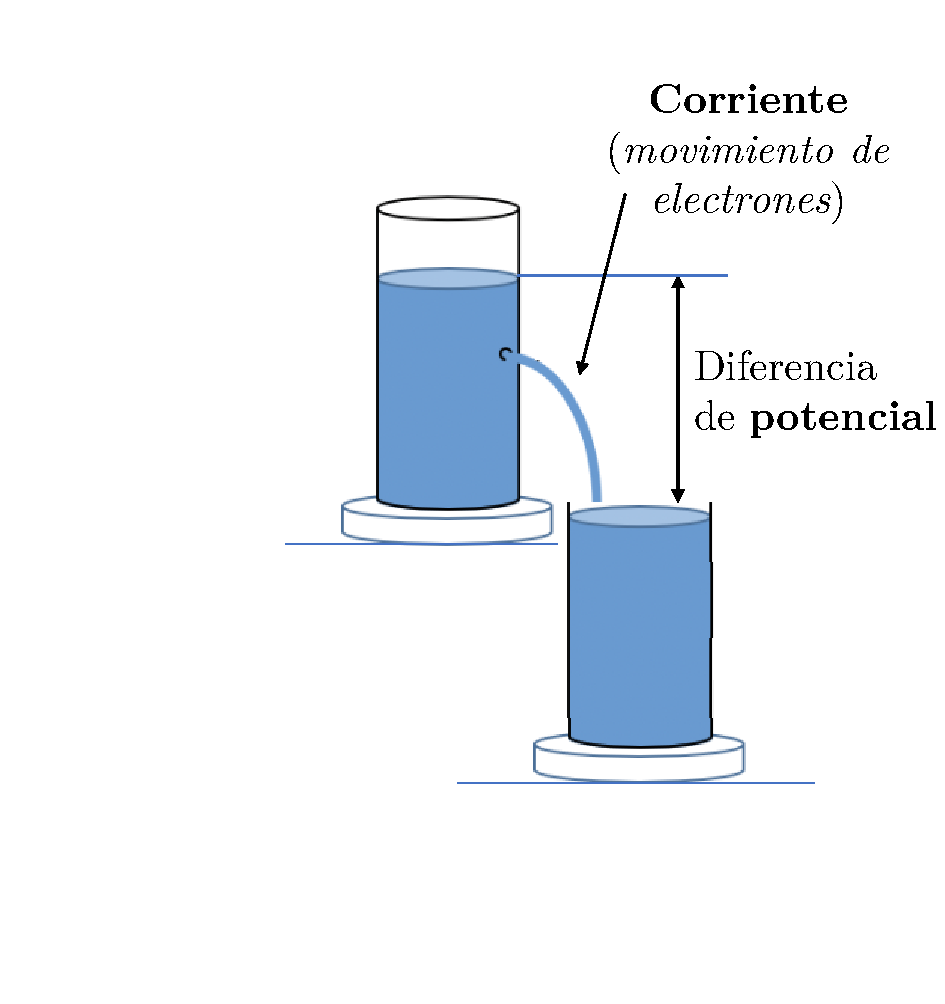
\includegraphics[height=0.9\textheight]{../figs/analogia_gravedad1.pdf}
    \end{column}
    \end{columns}
\end{frame}

%%%%%%%%%%%%%%%%%%

\begin{frame}{Potencial eléctrico y corriente eléctrica: \hspace{5mm}analogía con la gravedad}
    \begin{columns}
    \begin{column}{0.5\columnwidth}

        \vspace{-25mm}
        
        \begin{itemize}
         \item Las dos magnitudes principales en esta asignatura son la diferencia de \alert{potencial eléctrico} (o \textit{tensión}) y la \alert{corriente eléctrica} (o \textit{intensidad})

        \vspace{5mm}
        
        \item Para entender estas magnitudes de forma visual, podemos establecer un \alert{paralelismo con la gravedad}:
        \end{itemize}
    \end{column}  
    \begin{column}{0.5\columnwidth}
        \vspace{5mm}
        
        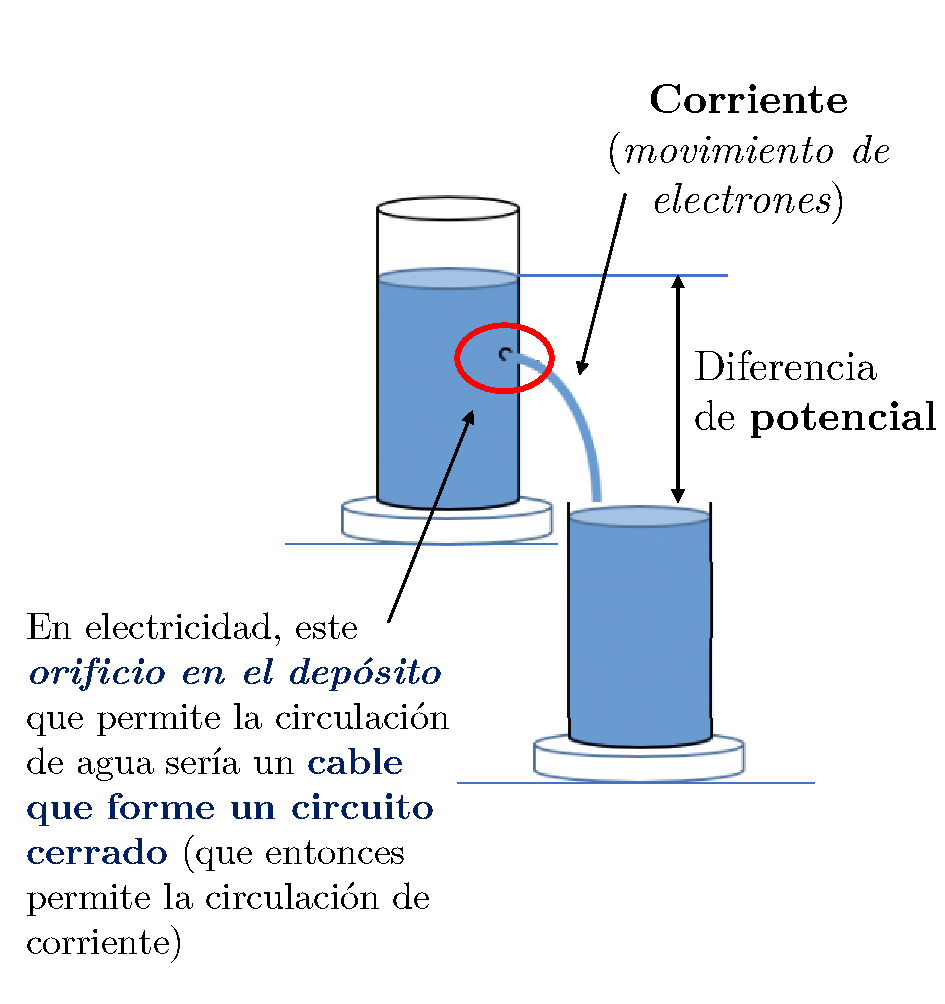
\includegraphics[height=0.9\textheight]{../figs/analogia_gravedad2.pdf}
    \end{column}
    \end{columns}
    
    
\end{frame}

%%%%%%%%%%%%%%%%%%

\begin{frame}{¿Qué aplicaciones tiene esta asignatura?}

    Los modelos matemáticos que vamos a estudiar en Teoría de Circuitos se usan en:
    % https://en.wikipedia.org/wiki/Network_analysis_(electrical_circuits)
    
    \begin{itemize}
        \item Circuitos de gran tamaño: \alert{sistemas eléctricos de potencia}
        \item Circuitos de pequeño tamaño: \alert{circuitos electrónicos}        
    \end{itemize}
    % Aunque con algunas limitaciones, por ejemplo cuando aparecen elementos no lineales

    \vspace{5mm}

    \begin{columns}
    \begin{column}{0.4\columnwidth}
        \begin{center}
            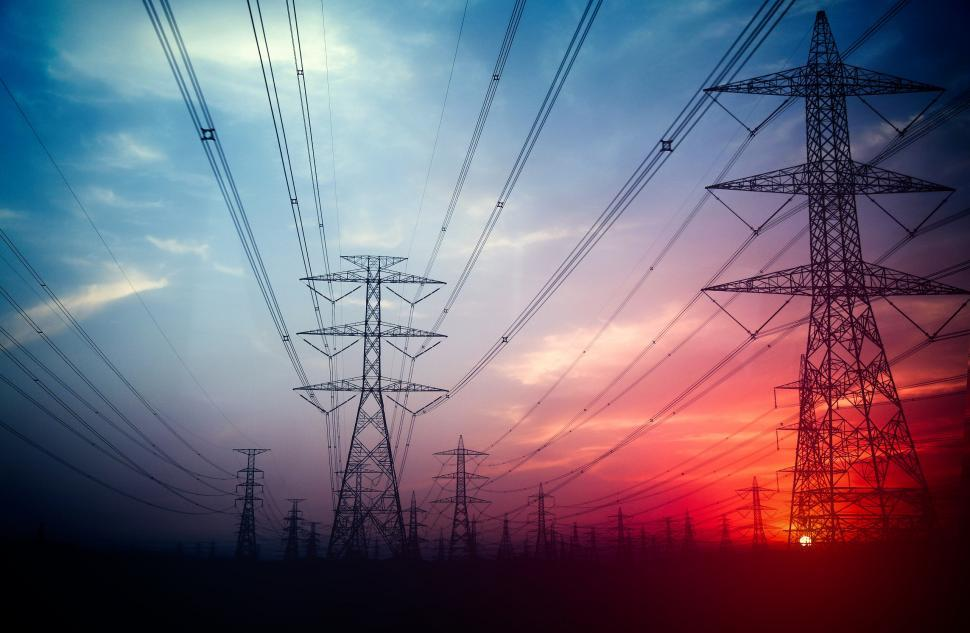
\includegraphics[height=0.4\textheight]{../figs/power_lines.jpg}
        \end{center}
    \end{column}  
    \begin{column}{0.4\columnwidth}
        \begin{center}
            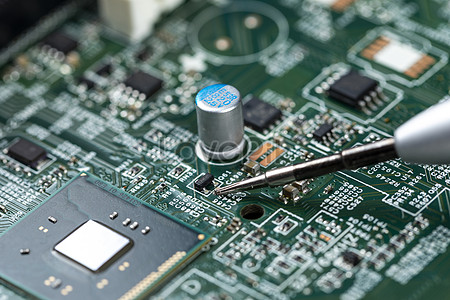
\includegraphics[height=0.4\textheight]{../figs/electronic_circuit.jpg}
        \end{center}
    \end{column}
    \end{columns}

\end{frame}

%%%%%%%%%%%%%%%%%%


\section{Conceptos fundamentales}

\begin{frame}{}
\vspace{15mm}
    \begin{center}
        \fbox{ \begin{minipage}{0.8\linewidth} 
        \begin{center}
            Esta asignatura está dedicada al \alert{análisis} de \alert{circuitos} 
            
            \alert{eléctricos} \alert{lineales} de \alert{parámetros concentrados}
        \end{center} 
        \end{minipage} }

        \vspace{15mm}

        (ahora entenderemos qué significan estos conceptos)
    \end{center}            
\end{frame} 

%%%%%%%%%%%%%%%%%%

\begin{frame}{Circuito eléctrico}
    \begin{minipage}[c]{0.62\linewidth}
        Un \alert{circuito eléctrico} es un conjunto de componentes eléctricos interconectados que crean un \alert{camino cerrado} por el que puede circular corriente eléctrica 
        \vspace{6mm}
        
        Incluye:
        
        \vspace{3mm}
        \begin{itemize}
        \item \alert{Elementos activos} (generadores): motivan la circulación de corriente

        \vspace{2mm}
        \item \alert{Elementos pasivos} (receptores): transforman o almacenan la energía eléctrica
        \end{itemize}
    \end{minipage}
    \hfill%
    \begin{minipage}[c]{0.3\linewidth}
        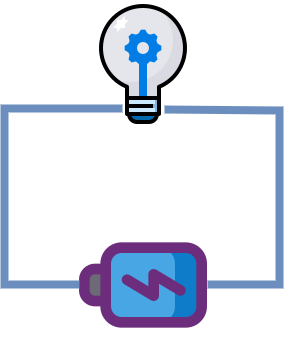
\includegraphics[width=\linewidth]{../figs/circuito.png}
    \end{minipage}
\end{frame}

%%%%%%%%%%%%%%%%%%

\begin{frame}{Análisis vs. diseño}
    El \alert{análisis} (o resolución) de un circuito eléctrico existente persigue determinar sus condiciones de funcionamiento:
    \begin{enumerate}
    \item Definir las \underline{ecuaciones correspondientes} al circuito

    \vspace{2mm}
    \item Obtener los \underline{valores de determinadas variables} importantes, a partir de dichas ecuaciones
    \end{enumerate}
    
    \vspace{6mm}
    
    El \alert{diseño} (o síntesis) de un circuito eléctrico tiene como objetivo definir el circuito eléctrico, es decir, determinar los componentes necesarios y su interconexión, para obtener unas condiciones de funcionamiento

    \vspace{1mm}
    
    \noindent\rule{\textwidth}{0.5pt}

    \vspace{1mm}
    
    En esta asignatura \alert{NO} vamos a diseñar circuitos, únicamente \alert{los analizaremos}
\end{frame}

%%%%%%%%%%%%%%%%%%

\begin{frame}{Sistemas lineales}
    Todos los circuitos eléctricos que se estudian en esta asignatura se comportan como \alert{sistemas lineales}: 
    
    \vspace{5mm}
    \begin{itemize}
    \item \(f(x + y) = f(x) + f(y)\)
    
    La respuesta \(f\) a la suma de dos entradas \(x\) e \(y\) es igual a la suma de la respuesta individual a cada una de las entradas
    
    \vspace{5mm}
    \item \(f(k \cdot x) = k \cdot f(x)\)
    
    La respuesta a una entrada que está multiplicada por un factor de escala \(k\) es igual a multiplicar por este factor a la respuesta a la entrada
    \end{itemize}
\end{frame}

%%%%%%%%%%%%%%%%%%

\begin{frame}{Parámetros concentrados}
    \begin{itemize}
        \item \alert{No nos preocupan las dimensiones espaciales} del circuito
        
        \vspace{3mm}
        Por ejemplo, una pila alcalina y una central nuclear pueden modelarse ambas como fuentes de tensión (la primera de 1,5 V y la segunda de 20 kV)
        %  La forma más rigurosa de explicar parámetros concentrados es decir que un cable de varios kilómetros de longitud de representa únicamente como una resistencia. Pero creo que esto es algo más confuso al principio de la asignatura, porque consideramos los cables como ideales, sin resistencia.
    \end{itemize}    

    \begin{columns}
    \begin{column}{0.4\columnwidth}
        \begin{column}{0.2\columnwidth}
        \begin{center}
            \hspace*{-12mm}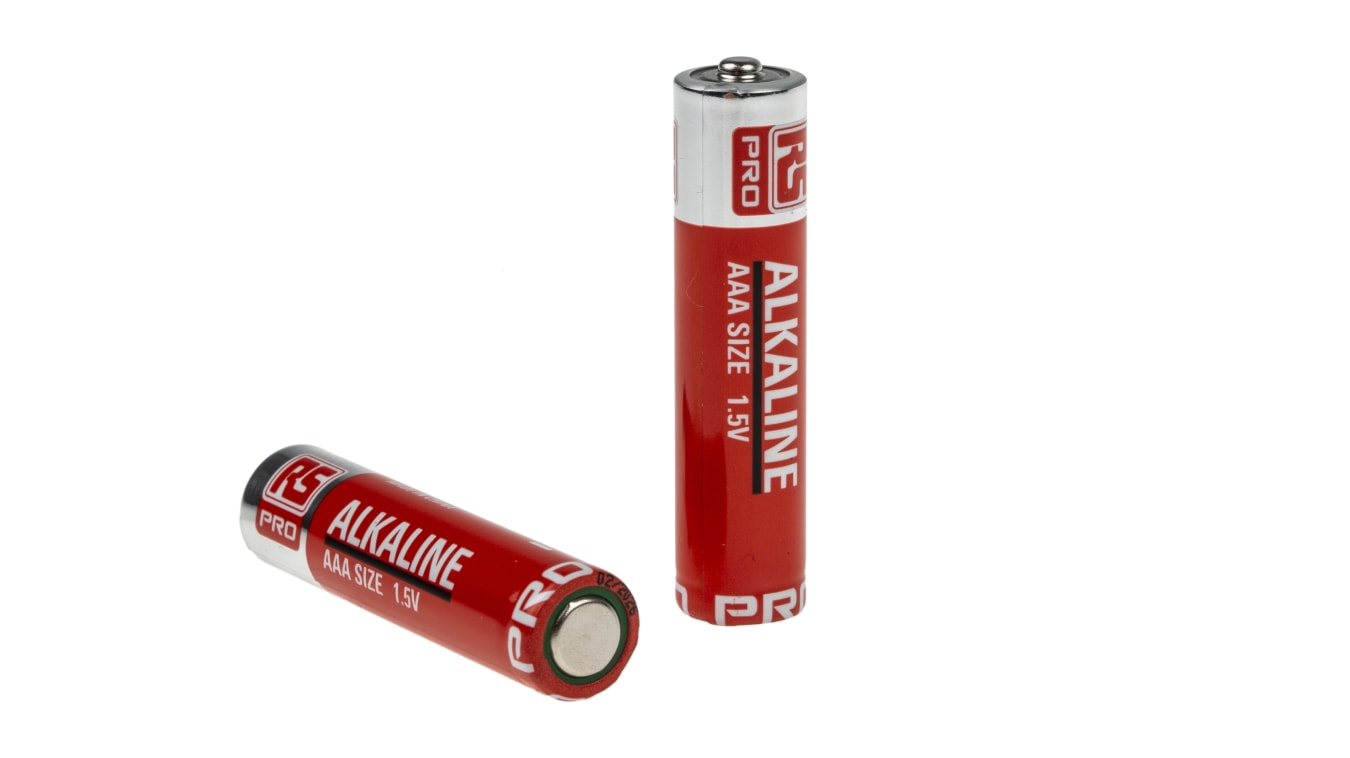
\includegraphics[height=0.4\textheight]{../figs/pila_alcalina.jpg} 
        \end{center}
        \end{column}  
        \begin{column}{0.05\columnwidth}
            \hspace*{2mm}\scalebox{2}{$\rightarrow$} % https://tex.stackexchange.com/questions/3703/make-equations-large
        \end{column} 
        \begin{column}{0.3\columnwidth}
            \hspace*{-5mm}\includegraphics[height=0.3\textheight]{../figs/FuenteTension_DC_1V.pdf}
        \end{column}         
    \end{column}      
    \vrule
    \begin{column}{0.6\columnwidth}
        \begin{column}{0.35\columnwidth}
        \begin{center}
            \hspace*{5mm}\includegraphics[height=0.4\textheight]{../figs/central_nuclear.jpg} 
        \end{center}
        \end{column}  
        \begin{column}{0.05\columnwidth}
            \hspace*{4mm}\scalebox{2}{$\rightarrow$} % https://tex.stackexchange.com/questions/3703/make-equations-large
        \end{column} 
        \begin{column}{0.2\columnwidth}
            \hspace*{-9mm}\includegraphics[height=0.3\textheight]{../figs/FuenteTension_AC_20kV.pdf}
        \end{column} 
    \end{column}  
    \end{columns}
    
\end{frame}

%%%%%%%%%%%%%%%%%%

\begin{frame}{Parámetros concentrados: \hspace{5mm} ¿cuándo puede aplicarse?}

    \vspace{2mm}
    \begin{itemize}
        \item El modelo de parámetros concentrados nos permite simplificar las ecuaciones del electromagnetismo de Maxwell (lo que \alert{simplifica mucho los cálculos})
        \vspace{2mm}
        \item Es aplicable únicamente cuando \alert{las dimensiones del circuito son muy inferiores a la longitud de onda} de la señal que circula por el circuito
        \vspace{5mm}
    \end{itemize}

    \vspace{-1mm}
    \begin{columns}[T]
    \begin{column}{0.4\columnwidth}
        \alert{Válido} en redes eléctricas
        \begin{itemize}
            \item \alert{Frecuencia}: \SI{50}{\hertz} (en Europa)
            \item \alert{Longitud onda}: $6.000$\,\si{\kilo\meter}
            % λ = C/f, where λ is the wavelength (in meters), "C" is the speed of light (299,792,458 m/s), and "f" is the frequency (in Hz)
        \end{itemize}    
        % Por lo tanto, aplica para circuitos con longitudes de hasta unos 250 km (que todavía son 20 veces menores que la longitud de onda de 6.000 km).
        \begin{center}
            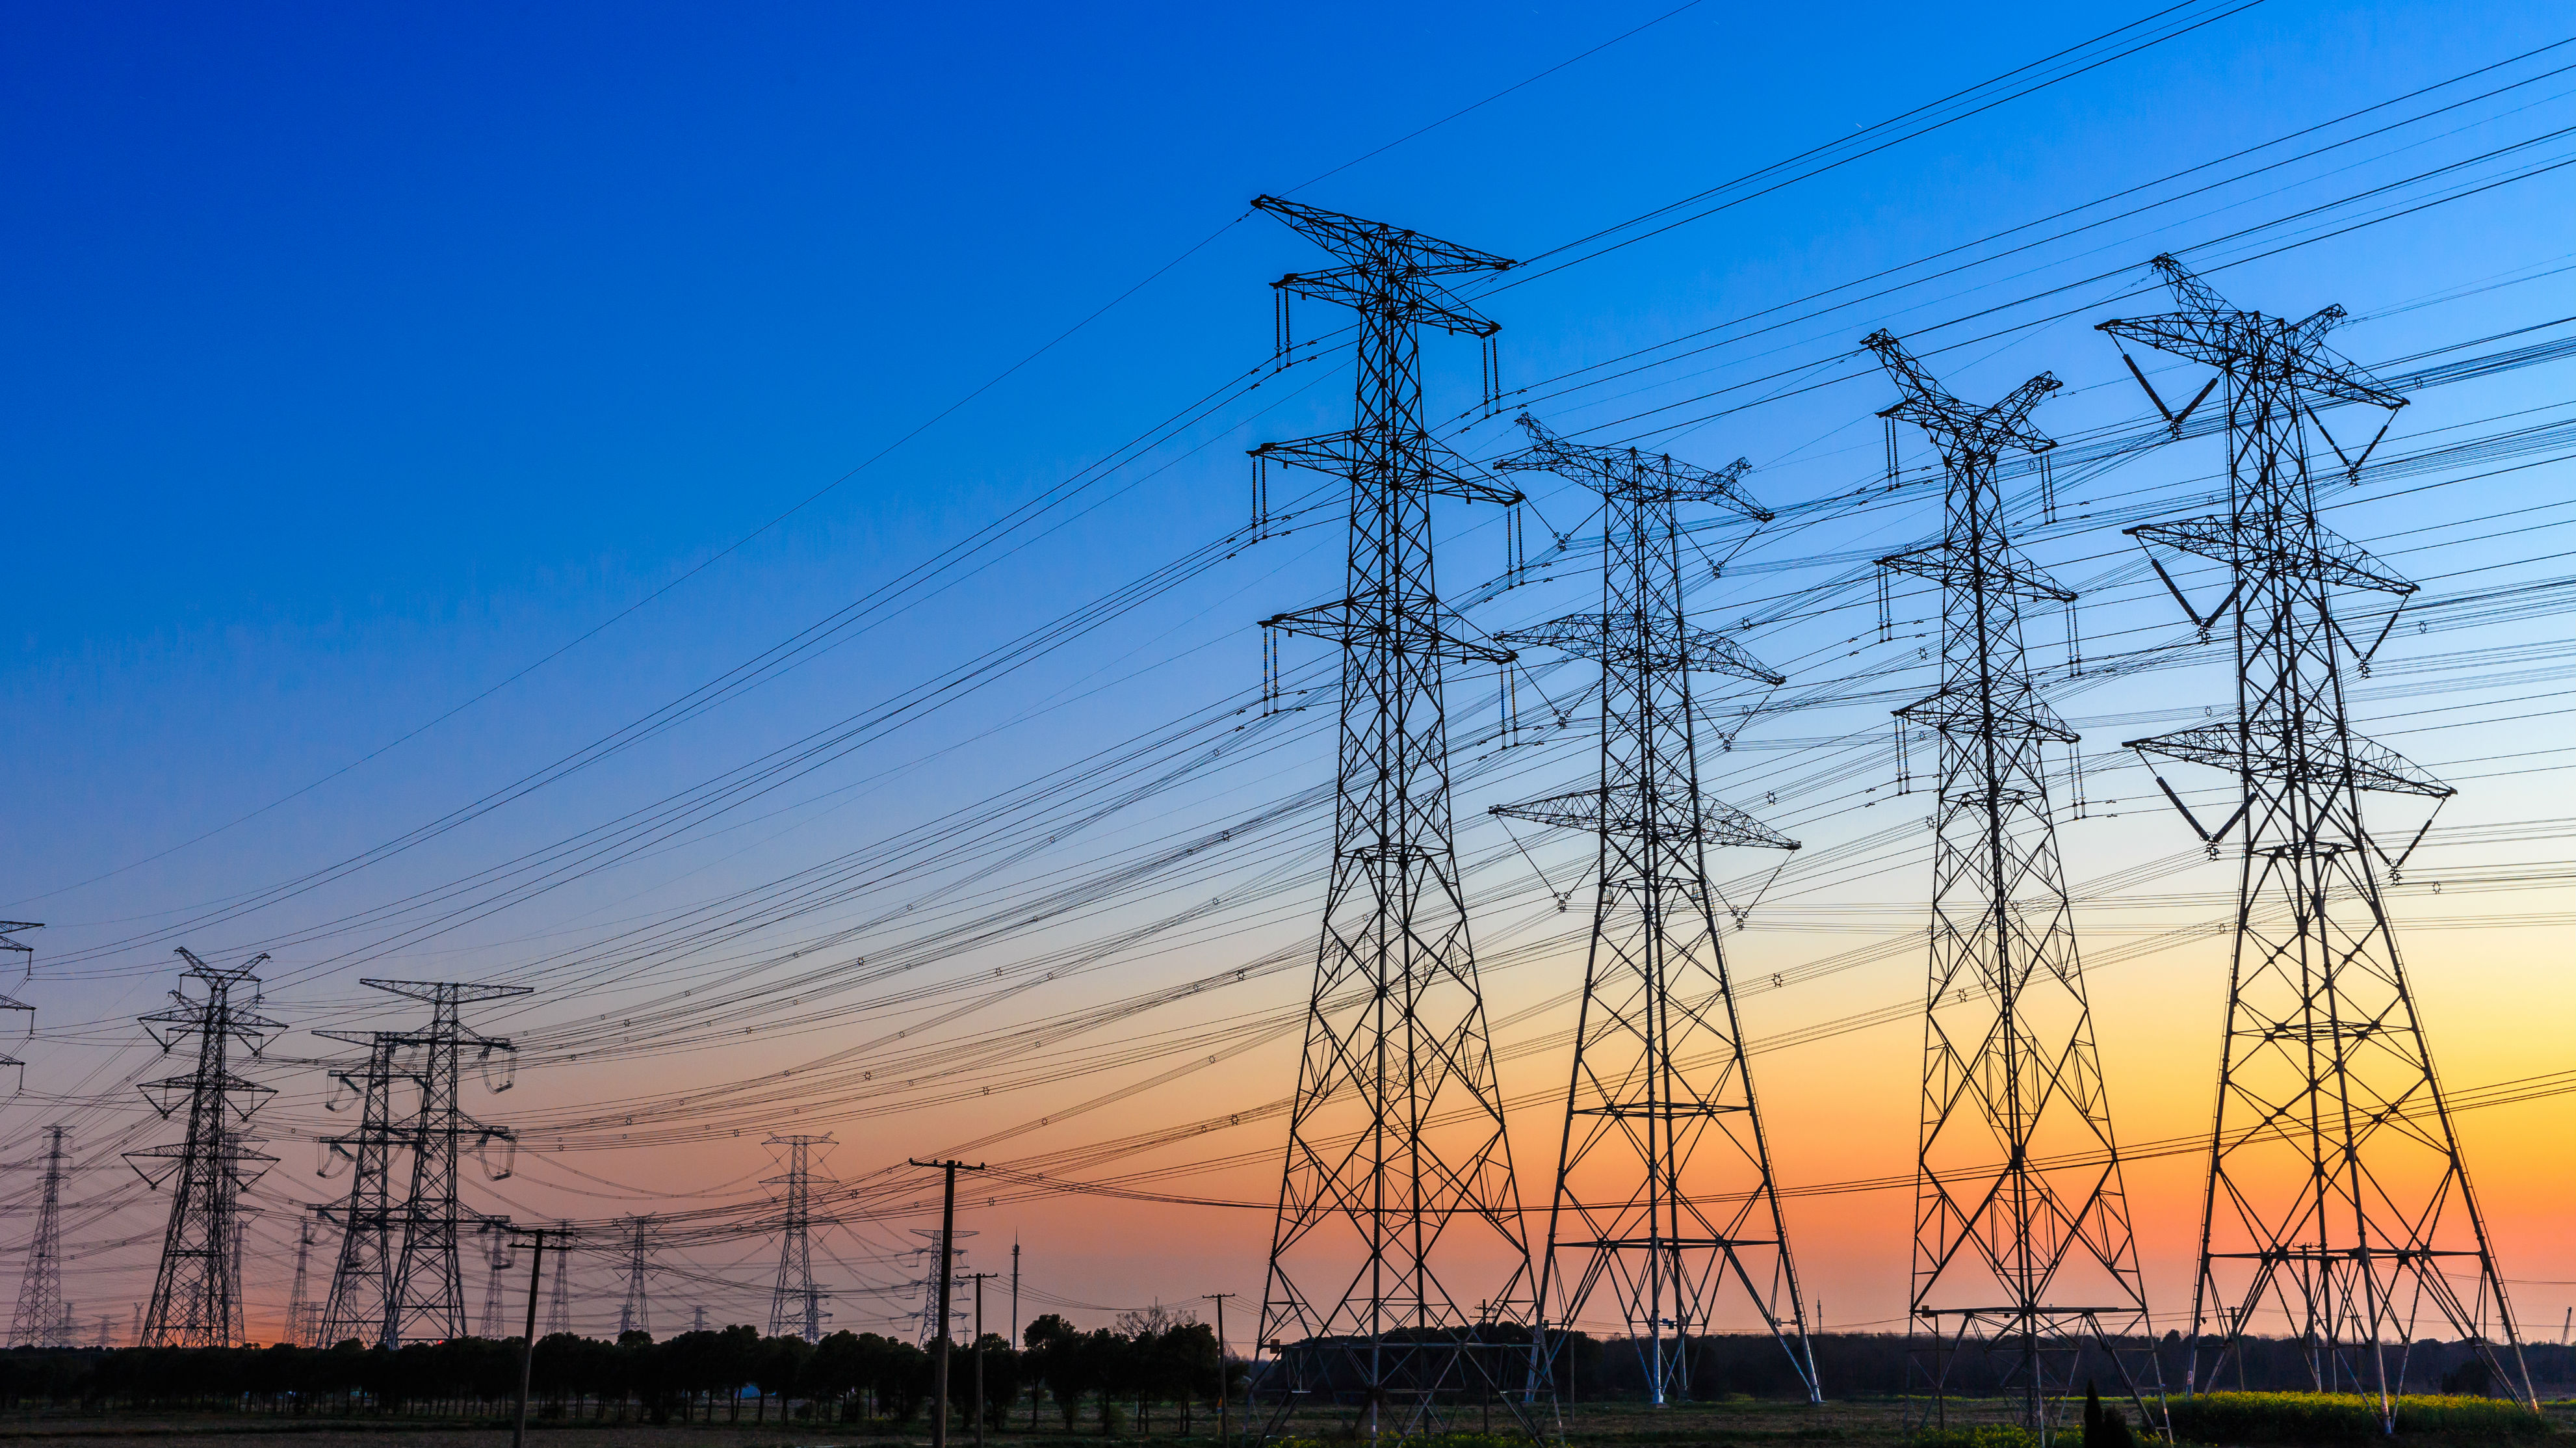
\includegraphics[height=0.35\textheight]{../figs/red_electrica.jpg} 
        \end{center}        
    \end{column}  
    \vrule
    \begin{column}{0.01\columnwidth}
    \end{column}     
    \begin{column}{0.49\columnwidth}
        \alert{\textcolor{red}{No válido}} en telecomunicaciones
        \begin{itemize}
            \item \alert{Frecuencia}: \SI{26}{\giga\hertz} (telefonía 5G)
            \item \alert{Longitud onda}: \SI{11.5}{\milli\meter}
        \end{itemize}
        % Como los circuitos de interés en telecomunicaciones son de muchos km de longitud, esta distancia es mucho mayor a la longitud de onda, así que no se puede aplicar parámetros concentrados.
        \begin{center}
            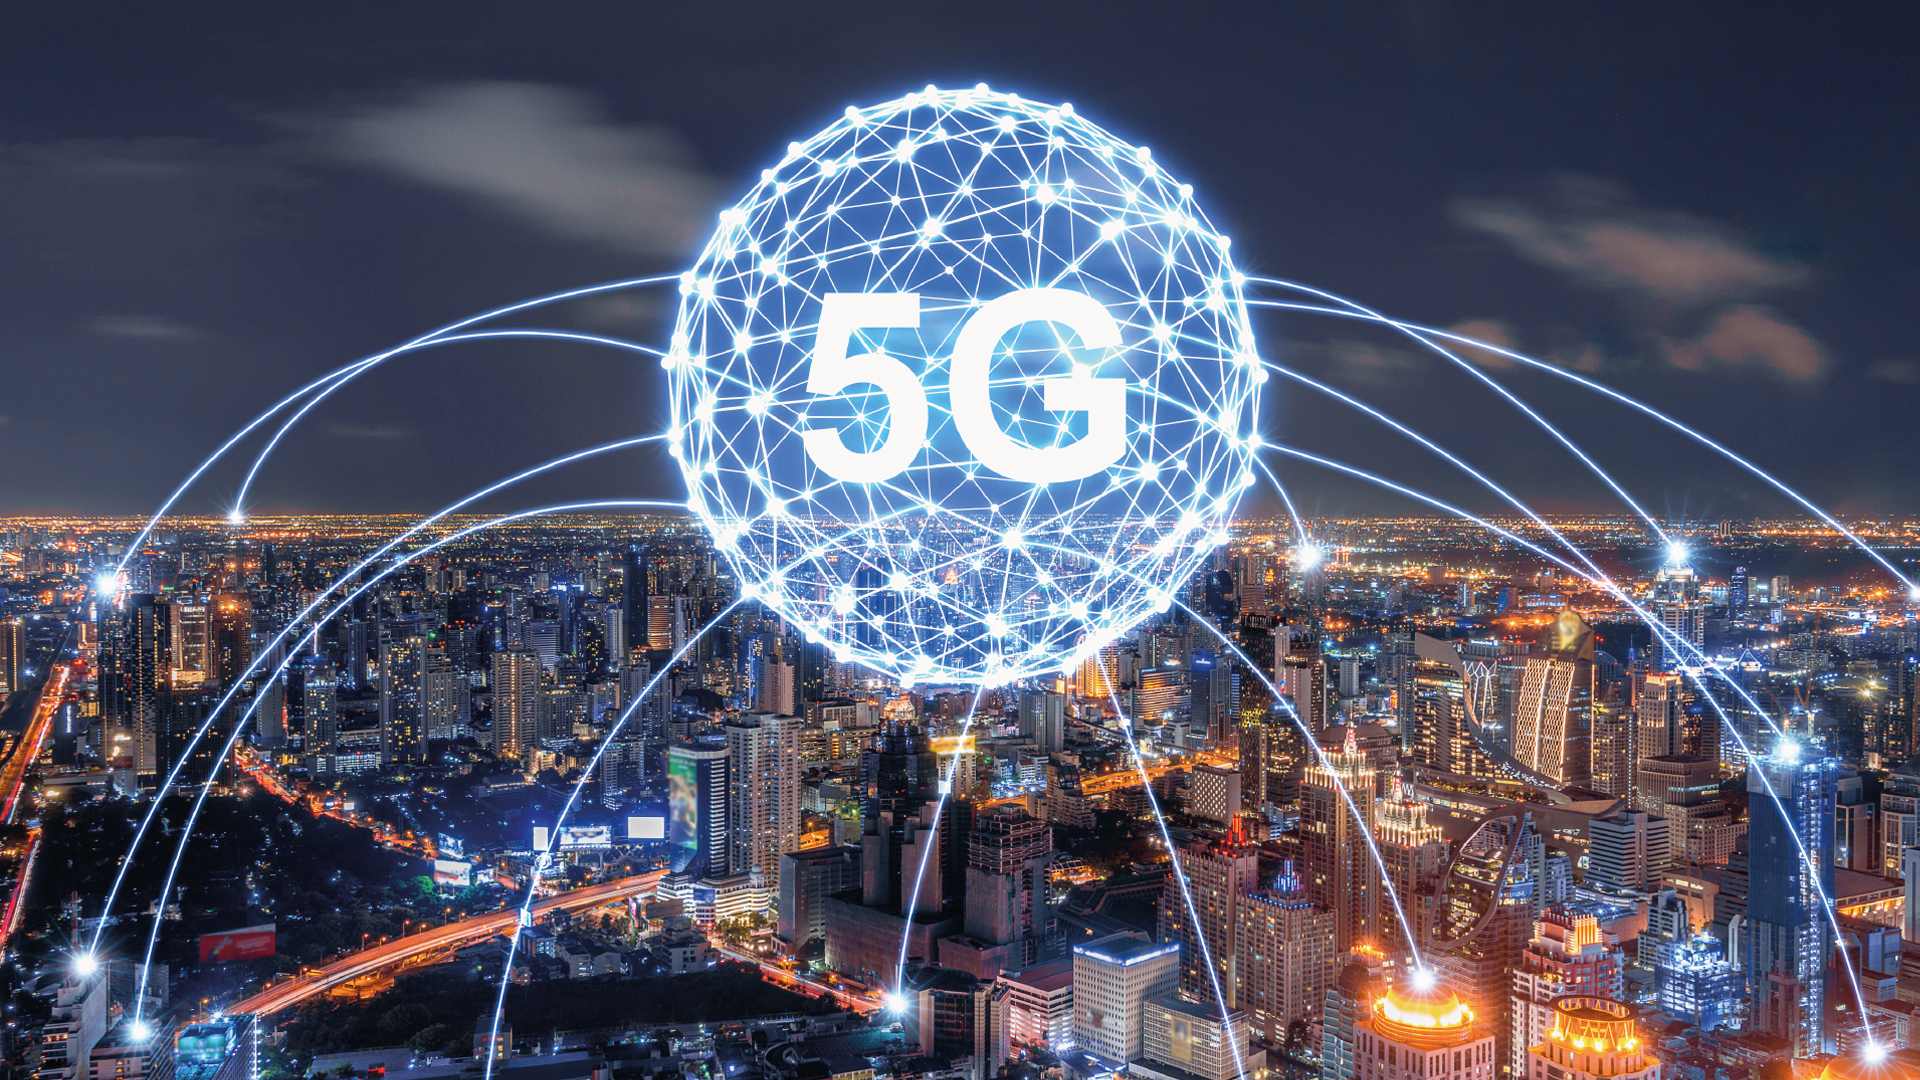
\includegraphics[height=0.3\textheight]{../figs/5G.jpg} 
        \end{center}
    \end{column}  
    \end{columns}
    
\end{frame}

%%%%%%%%%%%%%%%%%%

\subsection{Variables}

\begin{frame}{Variables}
    Las principales \alert{variables} con las que se trabaja en los circuitos eléctricos son:
    \vspace{5mm}
    \begin{itemize}
        \item Corriente eléctrica (o \textit{intensidad}, o \textit{amperaje})
        \vspace{2mm}
        \item Tensión eléctrica (o \textit{diferencia de potencial}, o \textit{voltaje})
        \vspace{2mm}
        \item Potencia eléctrica
        \vspace{2mm}
        \item Energía eléctrica
    \end{itemize}    
\end{frame}

%%%%%%%%%%%%%%%%%%

\begin{frame}{Corriente eléctrica}
    La \alert{intensidad de la corriente eléctrica} es la variación de la carga \(q(t)\) que atraviesa la sección transversal de un conductor por unidad de tiempo:
    \vspace{7mm}
    
    \begin{minipage}[c]{0.48\linewidth}
    \begin{equation*}
      i(t)=\frac{dq(t)}{dt}
    \end{equation*}
    \end{minipage}
    \hfill
    \begin{minipage}[c]{0.48\linewidth}
    \begin{center}
    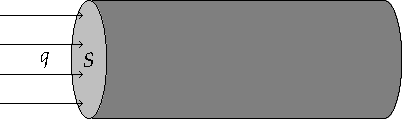
\includegraphics[width=0.8\linewidth]{../figs/seccion_conductor.pdf}
    \end{center}
    \end{minipage}
    
    \vspace{7mm}
    Se produce por el \alert{movimiento de electrones} (de $-$ a $+$)
    
    Sin embargo, por razones históricas, el convenio es considerar el \alert{movimiento de cargas positivas} (de $+$ a $-$)
    
    \vspace{3mm}
    La \alert{unidad} de la corriente es el \alert{amperio} [A] (culombios/segundo)

\end{frame}

%%%%%%%%%%%%%%%%%%

\begin{frame}{Corriente Continua (CC) y Corriente Alterna (CA)}
    \vspace{1mm}
    \begin{itemize}
        \item \alert{Corriente Continua}: siempre en el mismo sentido 

        \vspace{1mm}
        Caso particular, corriente constante \hspace{2mm}(\(\frac{d}{dt} = 0\)):
    \end{itemize}
    \begin{center}
        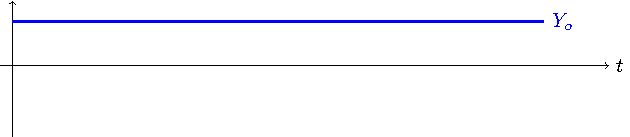
\includegraphics[height=0.25\textheight]{../figs/continua.pdf}
    \end{center}
    \vspace{-4mm}
    \begin{itemize}
        \item \alert{Corriente Alterna}: sentido cambiante 

        \vspace{1mm}
        Caso particular, corriente senoidal:
    \end{itemize}
    \begin{center}
        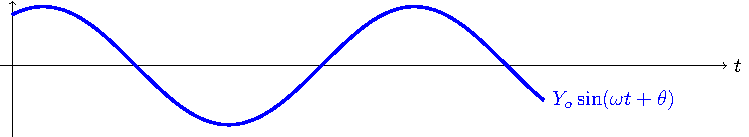
\includegraphics[height=0.25\textheight]{../figs/sin.pdf}
    \end{center}
\end{frame}

%%%%%%%%%%%%%%%

\begin{frame}{Corriente Continua (CC) y Corriente Alterna (CA)}
{Otros casos particulares (no estudiados en esta asignatura)}

    \vspace{1mm}
    \begin{itemize}
        \item Corriente \alert{Continua con rizado} (obtenida a partir de alterna trifásica rectificada):
    \end{itemize}
    \begin{center}
        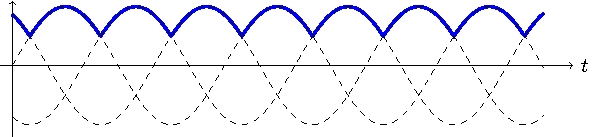
\includegraphics[height=0.25\textheight]{../figs/CA_rectificada.pdf}
    \end{center}
    \vspace{-4mm}
    \begin{itemize}
        \item Corriente \alert{Alterna con harmónicos} (obtenida con un inversor CC-CA):
    \end{itemize}
    \begin{center}
        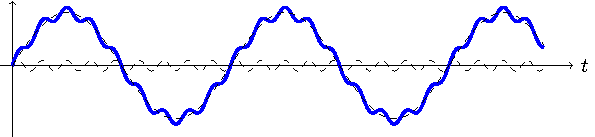
\includegraphics[height=0.25\textheight]{../figs/CA_armonicos.pdf}
    \end{center}
\end{frame}

%%%%%%%%%%%%%%%

\begin{frame}{Tensión eléctrica y f.e.m.}
    El \alert{potencial eléctrico en un punto}, \(v(t)\),  es la energía potencial que tiene una carga unitaria en ese punto, debida al campo eléctrico
    
    La \alert{tensión} o \alert{diferencia de potencial entre dos puntos} A y B, \(u_{AB}(t)\), es el trabajo realizado por el campo eléctrico al desplazar una carga unitaria entre esos puntos
    
    \begin{minipage}[c]{0.5\linewidth}
    \begin{equation*}
      u_{AB}(t) = v_A(t) - v_B(t) = \frac{dW_{e}}{dq}
    \end{equation*}
    \end{minipage}
    \hfill
    \begin{minipage}[c]{0.4\linewidth}
    \begin{center}
    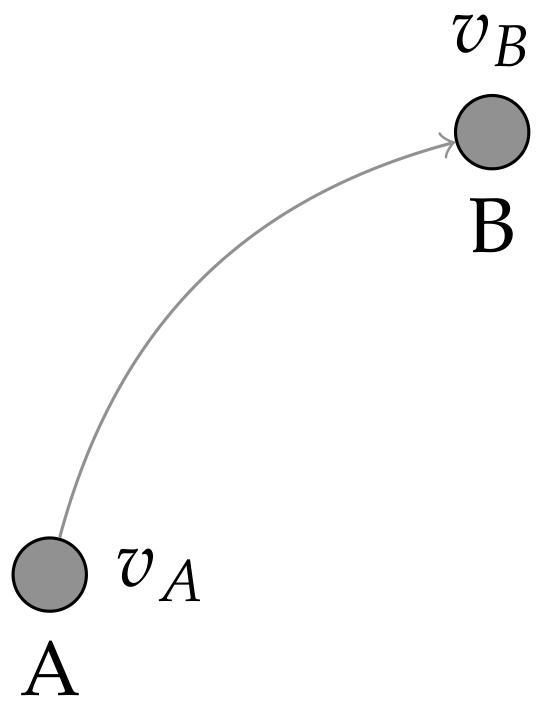
\includegraphics[height=0.3\textheight]{../figs/tension_puntos.PNG}
    \end{center}
    \end{minipage}
    
    La \alert{fuerza electromotriz} (f.e.m.) es la causa que mantiene a los electrones en movimiento (energía cedida por unidad de carga), y la proporcionan los elementos activos (\alert{generadores})
    
    La \alert{unidad} tanto de tensión eléctrica como de f.e.m. es el \alert{voltio} [V]
\end{frame}

%%%%%%%%%%%

\begin{frame}{La trayectoria no importa, pero el signo depende del sentido}
    \begin{minipage}[c]{0.6\linewidth}
        \begin{itemize}
        \item $u_{AB}(t)$ \alert{no depende de la trayectoria} del desplazamiento de los electrones, sino solo del potencial en cada punto $\rightarrow$ esto implica que el \alert{campo eléctrico} es \alert{conservativo}
        \vspace{12mm}
        \item Aunque la trayectoria no sea relevante, hay que tener en cuenta el \alert{sentido del desplazamiento}
    \end{itemize}
    \end{minipage}
    \hfill
    \begin{minipage}[c]{0.35\linewidth}
    \vspace{5mm}
    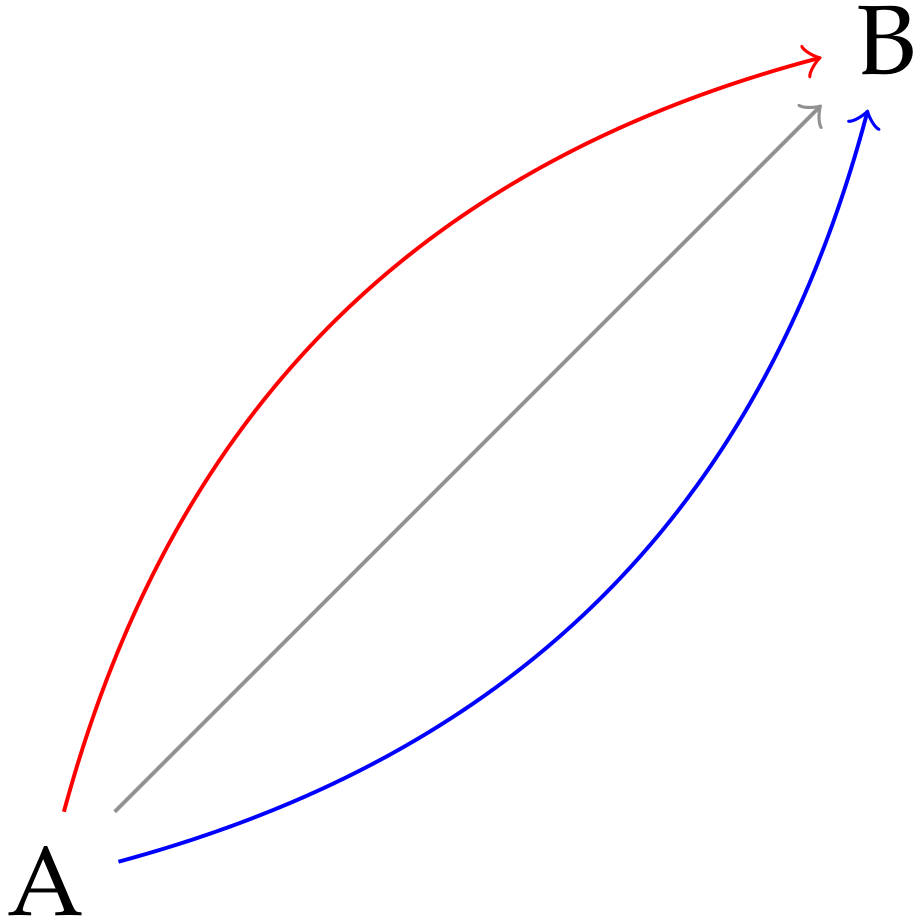
\includegraphics[width=0.5\linewidth]{../figs/diagrama_tension.PNG}
    
    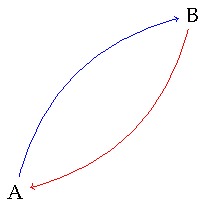
\includegraphics[width=0.5\linewidth]{../figs/sentido_tension.pdf}
    \end{minipage}
    
    Si el movimiento se produce desde B hasta A, el signo es contrario al anterior:
    \begin{equation*}
      u_{BA} = v_B - v_A = - u_{AB} 
    \end{equation*}
\end{frame}

%%%%%%%%%%%%%%%%

\begin{frame}{Potencia eléctrica}
    La \alert{potencia eléctrica} es la variación del trabajo del campo eléctrico por unidad de tiempo:
    
    \vspace{4mm}
    \begin{equation*}
      p(t)=\frac{dW_{e}}{dt}= \underbrace{\dfrac{dW_e}{dq(t)}}_{u(t)} \cdot \underbrace{\vphantom{\dfrac{dW_e}{dq(t)}} \dfrac{dq(t)}{dt}}_{i(t)} = \boxed{\vphantom{\dfrac{dq(t)}{dt}}  u(t) \cdot i(t)}
    \end{equation*}
    
    \vspace{4mm}
    La \alert{unidad} de la potencia eléctrica es el \alert{vatio} [W]
\end{frame}

%%%%%%%%%%%%%%%%

\begin{frame}{Signo de la potencia eléctrica}
    Para determinar el \alert{signo de la potencia eléctrica} hay que tener en consideración los signos de las variables de las que depende, la tensión y la corriente
    \vspace{5mm}
    \begin{itemize}
        \item Flechas en \alert{mismo sentido}: potencia \alert{positiva} % (absorbe potencia) $\rightarrow$ \alert{receptor}
        %\begin{itemize}
        %    \item {\normalsize La corriente \emph{entra} por el terminal de mayor potencial}
        %\end{itemize}

        \vspace{2mm}        
        \begin{center}
            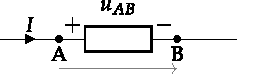
\includegraphics[height=0.17\textheight]{../figs/signo_potencia1.pdf}            
        \end{center}
    
    \vspace{5mm}
        \item Flechas en \alert{sentidos opuestos}: potencia \alert{negativa} % (genera potencia) $\rightarrow$ \alert{generador}
        %\begin{itemize}
        %    \item {\normalsize La corriente \emph{sale} por el terminal de mayor potencial}
        %\end{itemize}

        \vspace{2mm}  
        \begin{center}
            \hspace*{-7mm}
            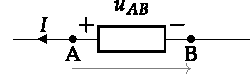
\includegraphics[height=0.17\textheight]{../figs/signo_potencia2.pdf}
        \end{center}
    \end{itemize}
\end{frame}

%%%%%%%%%%%%%%%%

\begin{frame}{Receptores y generadores}
    \vspace{2mm}
    Es habitual \alert{interpretar} el signo de la potencia en términos de potencia absorbida o potencia entregada
    
    \vspace{1mm}
    \begin{itemize}
        \item Un \alert{circuito receptor absorbe potencia} y la corriente \emph{entra} por el terminal de mayor potencial

        \vspace{2mm}
        \item Un \alert{circuito generador entrega potencia} y la corriente \emph{sale} por el terminal de mayor potencial
    \end{itemize}

    \vspace{-4mm}
    \begin{center}
        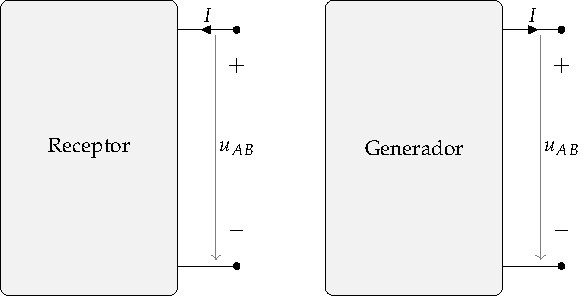
\includegraphics[height=0.5\textheight]{../figs/receptor_generador.pdf}
    \end{center}
\end{frame}

%%%%%%%%%%%%%%%%

\begin{frame}{Potencia y energía}
    \begin{description}    
        \item[{Energía}:] capacidad de un sistema para realizar un trabajo 
        
        \vspace{2mm}
        $E=P\cdot t$
        
        \vspace{2mm}
        Unidades: [J], [Wh], [kWh]
        
        % 1 kWh $=$ 3.6 MJ
        
        \vspace{5mm}
        
        \item[{Potencia}:] trabajo realizado por unidad de tiempo

        \vspace{2mm}
        
        Unidades: [W], [kW]
    \end{description}
\end{frame}

%%%%%%%%%%%%%%%%

\section{Elementos de los circuitos}

\subsection{Elementos pasivos}

\begin{frame}{Elementos pasivos en Teoría de Circuitos}
    Tres tipos de elementos pasivos en esta asignatura:
    \vspace{2mm}
    \begin{itemize}
        \item Resistencias         
        \vspace{2mm}
        \item Bobinas 
        \vspace{2mm}
        \item Condensadores
    \end{itemize}
\end{frame}

%%%%%%%%%%%%%%%%

\begin{frame}{Resistencia}
    \begin{itemize}
        \item \alert{\large Ley de Ohm}: 
        \vspace{2mm}
        
        Una resistencia $R$ provoca una \alert{diferencia de potencial} entre sus terminales \alert{directamente proporcional} a la corriente que la atraviesa
        
        \vspace{2mm}
        Unidades de resistencia: ohmios [\(\Omega\)] 
    \end{itemize}
    \vspace{3mm}
    \[
    \Large \boxed{u(t) = R \cdot i(t)}
    \]
    \begin{itemize}
        \item \alert{Criterio de signos}: la tensión es positiva en el terminal por el que entra la corriente (las flechas de tensión y corriente tienen el mismo sentido)
    \end{itemize}
    \begin{columns}
        \begin{column}{0.5\columnwidth}
            \begin{center}
            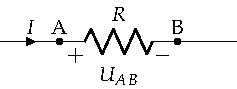
\includegraphics[height=0.2\textheight]{../figs/Resistencia.pdf}
            \end{center}
        \end{column}
        \begin{column}{0.5\columnwidth}
            \begin{center}
            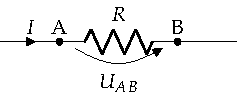
\includegraphics[height=0.2\textheight]{../figs/Resistencia_Flecha.pdf}
            \end{center}
        \end{column}
    \end{columns}
\end{frame}

%%%%%%%%%%%%%%%%

\begin{frame}{Resistividad}
    \begin{itemize}
        \item El valor de la resistencia depende de la \alert{resistividad del material} (\(\rho\)), de la \alert{sección} (\(S\)), y de la
        longitud (\(l\)):
    \end{itemize}
    \begin{equation*}
      R = \rho \cdot \frac{l}{S}
    \end{equation*}
    
    \begin{itemize}
        \item La \alert{sección} se expresa en \(\si{\milli\meter\squared}\)
        
        \vspace{4mm}
        \item La \alert{resistividad} depende del material conductor y de la temperatura ambiente:
        \vspace{2mm}
        \begin{itemize}
            \item \normalsize{Cobre a 20ºC: \(\qty{17.24}{\milli\ohm\milli\meter\squared\per\meter}\)}
            \vspace{2mm}
            \item La resistividad \alert{aumenta con la temperatura}: 
            
            los átomos del material vibran con mayor virulencia al subir la temperatura, y por tanto dificultan el flujo de electrones a través del material 
        \end{itemize}
    \end{itemize}
\end{frame}

%%%%%%%%%%%%%%%%

\begin{frame}{Cortocircuito y circuito abierto}
    \begin{itemize}
    \item \alert{Cortocircuito}: resistencia nula (tensión nula)
    \end{itemize}
    
    \begin{center}
    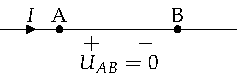
\includegraphics[height=0.2\textheight]{../figs/Cortocircuito.pdf}
    \end{center}
    
    \begin{itemize}
    \item \alert{Circuito abierto}: resistencia infinita (corriente nula)
    \end{itemize}
    
    \begin{center}
    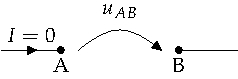
\includegraphics[height=0.2\textheight]{../figs/CircuitoAbierto.pdf}
    \end{center}
\end{frame}

%%%%%%%%%%%%%%%%

\begin{frame}{Ley de Joule}
    \begin{center}
    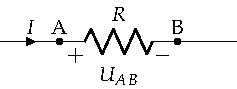
\includegraphics[height=0.2\textheight]{../figs/Resistencia.pdf}
    \end{center}
    
    \begin{itemize}
    \item \alert{Ley de Joule}: las resistencias disipan energía eléctrica produciendo \alert{calor}
    \end{itemize}
    
    
    \[
    \Large \boxed{p(t)=R\cdot i^{2}(t)}
    \]
\end{frame}

%%%%%%%%%%%%%%%%




\begin{frame}{Bobina o inductancia} \label{diapo:bobina_inicio}
    \begin{minipage}[c]{0.47\linewidth}     

        \vspace{5mm}
        Cualquier \alert{corriente} (ya sea constante o variable) \alert{crea un campo magnético} a su alrededor (ley de Ampère)
        
        \vspace{3mm}
        
        \begin{center}
            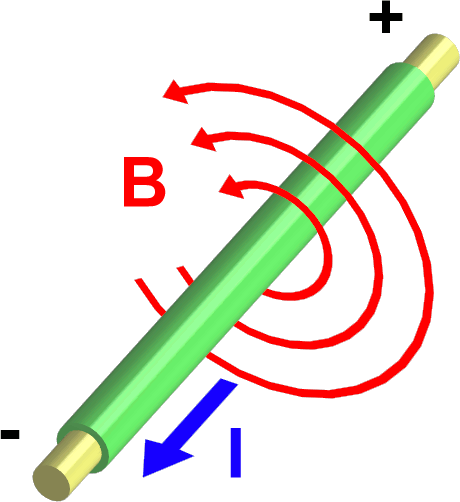
\includegraphics[height=0.5\textheight]{../figs/Electromagnetism.png}
        \end{center}
    \end{minipage}
    \hfill%
    \begin{minipage}[c]{0.47\linewidth}
    
        \vspace{3mm}
        Un \alert{conductor arrollado} crea una campo magnético más intenso: \alert{electroimán}
        % (cuantas más espiras, más intenso el campo magnético)
        % Un electroimán es una bobina por la que se hace circular una corriente. Con DC, también se crea un electroimán (lo que no hay es tensión inducida)
        \begin{center}
            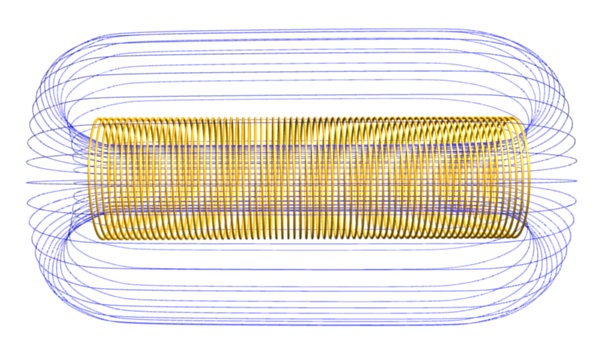
\includegraphics[height=0.5\textheight]{../figs/Solenoide.jpg}
        \end{center}
        % Las líneas de campo se suman para crear un campo magnético más intenso en el interior de la bobina
    \end{minipage}
\end{frame}

%%%%%%%%%%%%%%%%%%

\begin{frame}{Bobina o inductancia}

    \vspace{3mm}
    \alert{Bobina:} conductor arrollado alrededor de un núcleo
    \begin{center}
    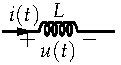
\includegraphics[height=0.2\textheight]{../figs/Bobina.pdf}
    \end{center}

    Cuando una corriente oscilante atraviesa una bobina, se produce una \alert{tensión inducida que se opone a dicha corriente} (ley de Faraday-Lenz)

    \begin{itemize}
        \item La tensión inducida es directamente \alert{proporcional al cambio de la corriente}: la constante de proporcionalidad es el coeficiente de autoinducción o \alert{inductancia} `$L$' (unidades: henrios [H])
    \end{itemize}
    \[
        \boxed{ u_L(t)=L\cdot\frac{di(t)}{dt} } %\rightarrow i(t_f)=i(t_i)+\dfrac{1}{L}\cdot\int_{t_i}^{t_f} u(t)\cdot dt
    \]
    
    %La inductancia $L$ expresa la relación entre el cambio de flujo magnético y el cambio de corriente:
    %\begin{equation*}
    %	L= \dfrac{d\phi(t)}{di(t)}
	%\end{equation*}
\end{frame}

%%%%%%%%%%%%%%%%

\begin{frame}{Bobina o inductancia}
    \begin{center}
    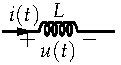
\includegraphics[height=0.2\textheight]{../figs/Bobina.pdf}
    \end{center}
    
    \begin{itemize}
    \item Almacena \alert{energía magnética}:
    \end{itemize}
    \[
      E_L(t) = \int_{-\infty}^t u(\tau) \cdot i(\tau) d\tau = \frac{1}{2} \cdot L \cdot i^2(t)
    \]
    \begin{itemize}
    \item En circuitos de CC es un \alert{cortocircuito}:
    \end{itemize}
    \begin{equation*}
      \frac{di(t)}{dt} = 0 \quad \Rightarrow \quad U_L = 0
    \end{equation*}
\end{frame}

%%%%%%%%%%%%%%%%

\begin{frame}{Condensador}
    \vspace{3mm}
    Material \alert{dieléctrico}: 
    
    %\vspace{1mm}
    \begin{itemize}
        \item Aislante eléctrico (material con baja conductividad), pero con una propiedad particular: sus \alert{moléculas se polarizan} en presencia de un campo eléctrico 
        % Debido a la polarización dieléctrica, se crea un campo eléctrico interno que reduce el campo general dentro del propio dieléctrico
    \end{itemize}

    \vspace{1mm}
    \alert{Ejemplos} de dieléctricos: aire, vidrio, papel
    
    \vspace{1mm}
    
    \begin{center}
        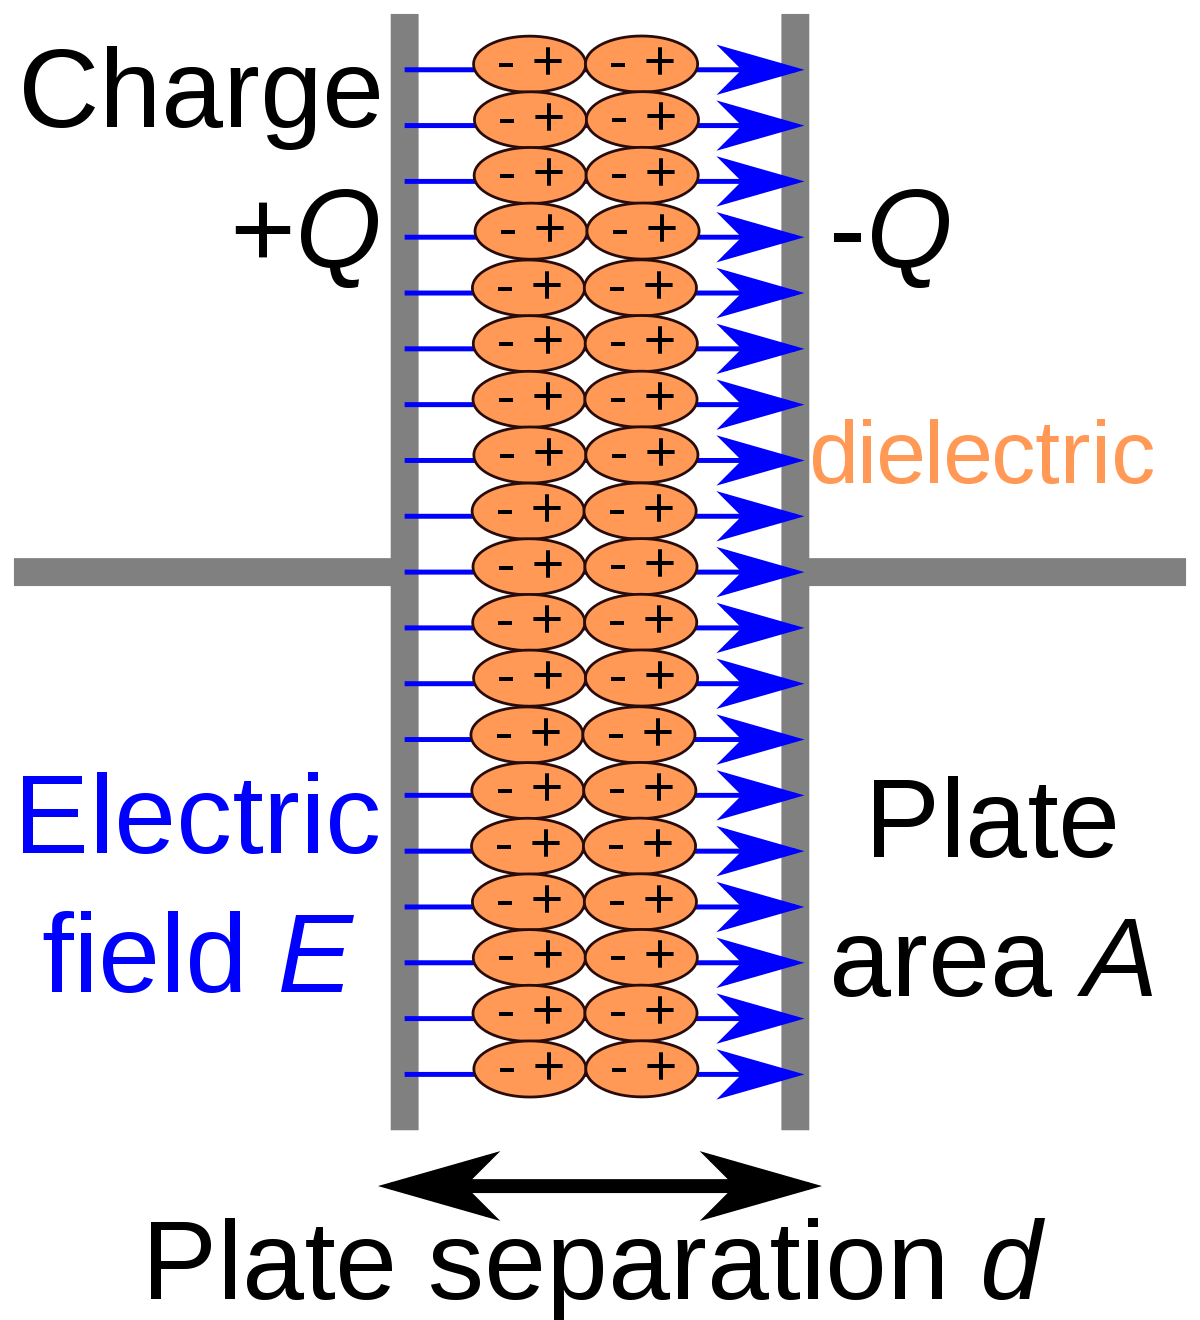
\includegraphics[height=0.55\textheight]{../figs/capacitor_dielectric.png}
    \end{center}
\end{frame}

%%%%%%%%%%%%%%%%
\begin{frame}{Condensador}

    \vspace{2mm}
    \alert{Condensador}: dos placas metálicas separadas por un material dieléctrico 
    
    Al aplicar tensión se produce una \alert{separación de cargas opuestas} que se \alert{acumulan} en cada placa
    \vspace{-2mm}
    \begin{center}
    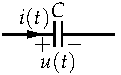
\includegraphics[height=0.2\textheight]{../figs/Condensador.pdf}
    \end{center}

    La \alert{carga acumulada} en un instante es \alert{proporcional} a la \alert{diferencia de potencial} en ese instante: la constante de proporcionalidad es la \alert{capacidad} (unidades: faradios [F]) % La capacidad depende de la geometría de las placas y del material dieléctrico usado
    \[
    q(t) = C \cdot u(t)
    \]
    
    \begin{itemize}
    \item En el proceso de carga se produce una corriente eléctrica entre las dos placas:
    \end{itemize}
    \begin{equation*}
        i_C(t) = \frac{dq(t)}{dt} = \boxed{ C \cdot \frac{du(t)}{dt} } %\rightarrow u(t_f)=u(t_i)+\dfrac{1}{C}\cdot\int_{t_i}^{t_f} i(t)\cdot dt
    \end{equation*}
\end{frame}

%%%%%%%%%%%%%%%%

\begin{frame}{Condensador}
    \begin{center}
    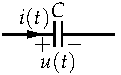
\includegraphics[height=0.2\textheight]{../figs/Condensador.pdf}
    \end{center}
    
    \begin{itemize}
    \item Un condensador almacena \alert{energía eléctrica}:
    \end{itemize}
    \[
      E_c(t) = \int_{-\infty}^t u(\tau) \cdot i(\tau) d\tau = \boxed{ \frac{1}{2} \cdot C \cdot u^2(t) }
    \]
    
    \begin{itemize}
    \item En un circuito de corriente continua se comporta como un \alert{circuito abierto}:
    \end{itemize}
    \begin{equation*}
      \frac{du(t)}{dt} = 0 \quad \Rightarrow \quad I_c = 0
    \end{equation*}

    \vspace{-3mm}
    \hyperlink{diapo:bobinas_serie}{.} % Sobre la cross-reference usando "hyperlink": https://tex.stackexchange.com/questions/70143/cross-reference-with-custom-text
\end{frame}

%%%%%%%%%%%%%%%%

\subsection{Elementos activos}

\begin{frame}{Generadores de tensión}
    Proporcionan una diferencia de potencial $U$ entre sus bornes de salida
    \vspace{-5mm}
    \begin{columns}[T]
    \begin{column}{0.4\columnwidth}
        \begin{center}
         \hspace*{-10mm}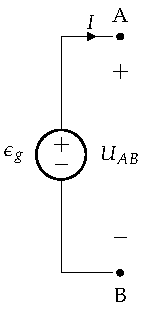
\includegraphics[height=0.5\textheight]{../figs/FuenteTensionIdealDC.pdf}  

        \vspace{2mm}  
        \alert{Ideal}: 
        
        impone tensión a la salida   
        
        \small{(la corriente depende del circuito)}
        \begin{equation*}
            u_{AB}=\epsilon_g
        \end{equation*}
        \end{center}
    \end{column}
    \begin{column}{0.38\columnwidth}
        \begin{center}
        \hspace*{-10mm}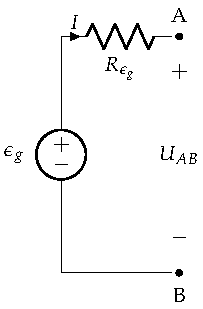
\includegraphics[height=0.5\textheight]{../figs/FuenteTensionRealDC.pdf}

        \vspace{2mm}        
        \alert{Real}: 
        
        con pérdidas, modeladas mediante una resistencia \alert{en serie}
        \vspace{-2mm}
        \begin{equation*}
            u_{AB}<\epsilon_g
        \end{equation*}
        \end{center}
    \end{column}
    \begin{column}{0.21\columnwidth}

        \vspace{10mm}Se caracterizan por su \alert{fuerza
        electromotriz} $\epsilon_g$ (voltios [V])
        \begin{align*}
            \Aboxed{\epsilon_g&=U_{AB}+R_{\epsilon_g}\cdot I}\\[4pt]
            P_g&=\epsilon_g\cdot I
            % P_p&=R_{\epsilon_g}\cdot I^2\\
            % P_u&=U_{AB}\cdot I
        \end{align*}
        \footnotesize{(estas expresiones se entenderán mejor cuando veamos las leyes de Kirchhoff)}
    \end{column}
    \end{columns}
\end{frame}

%%%%%%%%%%%%%%%%

\begin{frame}{Generadores de corriente}
    Proporcionan una corriente $I$
    \vspace{-5mm}
    \begin{columns}[T]
    \begin{column}{0.4\columnwidth}
        \begin{center}
         \hspace*{-10mm}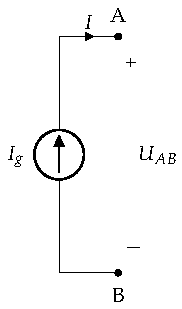
\includegraphics[height=0.5\textheight]{../figs/FuenteCorrienteIdeal.pdf}  

        \vspace{2mm}
        \alert{Ideal}: 
        
        impone corriente a la salida 
        
        \small{(la tensión depende del circuito)}
        \begin{equation*}
            I=I_g
        \end{equation*}
        \end{center}
    \end{column}
    \begin{column}{0.38\columnwidth}
        \begin{center}
        \hspace*{-10mm}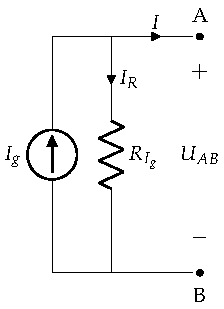
\includegraphics[height=0.5\textheight]{../figs/FuenteCorrienteRealDC.pdf}
        
        \vspace{2mm}
        \alert{Real}: con pérdidas, 
        
        modeladas mediante una resistencia \alert{en paralelo}
        \vspace{-2mm}
        \begin{equation*}
            I<I_g
        \end{equation*}
        \end{center}
    \end{column}
    \begin{column}{0.21\columnwidth}

        \vspace{10mm}Se caracterizan por su \alert{corriente de generador} $I_g$ (amperios [A])        
        \begin{align*}
            \Aboxed{I_g&=I+\dfrac{U_{AB}}{R_{I_g}}}\\
            P_g&=U_{AB}\cdot I_g
            %P_p&=\dfrac{U_{AB}^2}{R_{I_g}}\\
            %P_u&=U_{AB}\cdot I            
        \end{align*}
        \footnotesize{(estas expresiones se entenderán mejor cuando veamos las leyes de Kirchhoff)}
    \end{column}
    \end{columns}
\end{frame}

%%%%%%%%%%%%%%%%

\begin{frame}{Equivalencia de fuentes}
    \begin{columns}
    \begin{column}{0.25\columnwidth}
        \begin{center}
        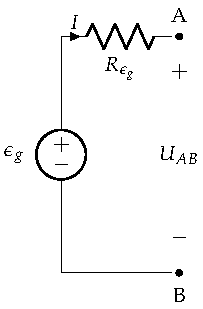
\includegraphics[height=0.5\textheight]{../figs/FuenteTensionRealDC.pdf}
        \end{center}
    \end{column}
    
    \begin{column}{0.48\columnwidth}
        \begin{itemize}
        \item Dos fuentes son equivalentes cuando suministran el mismo valor de tensión y corriente a un \alert{circuito externo}, para cualquier circuito

        \vspace{8mm}
        
        \item Sólo es posible establecer equivalencia entre \alert{fuentes reales}
        \end{itemize}
    \end{column}
    
    \begin{column}{0.25\columnwidth}
        \begin{center}
        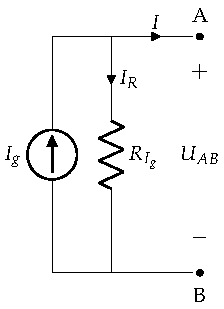
\includegraphics[height=0.5\textheight]{../figs/FuenteCorrienteRealDC.pdf}
        \end{center}
    \end{column}
    \end{columns}
\end{frame}

%%%%%%%%%%%%%%%%

\begin{frame}{Equivalencia de fuentes}
    \vspace*{5mm}
    \begin{columns}

    \begin{column}{0.5\columnwidth}
    \centering 
    La \alert{corriente en cortocircuito} 
    
    debe ser la misma:
    
        \begin{column}{0.25\columnwidth}
            \includegraphics[height=0.43\textheight]{../figs/FuenteTensionRealDC_SC.pdf}        
        \end{column}
        \begin{column}{0.25\columnwidth}
           \includegraphics[height=0.43\textheight]{../figs/FuenteCorrienteRealDC_SC.pdf}           
        \end{column}       
        \hfill
    \end{column}    
    \vrule
    \begin{column}{0.5\columnwidth}
    \centering 
    Y la \alert{tensión en circuito abierto} 
    
    debe ser la misma:
    
        \begin{column}{0.25\columnwidth}
            \hspace*{6mm}\includegraphics[height=0.43\textheight]{../figs/FuenteTensionRealDC_OC.pdf}        
        \end{column}
        \begin{column}{0.25\columnwidth}
           \includegraphics[height=0.43\textheight]{../figs/FuenteCorrienteRealDC_OC.pdf}
        \end{column}
        \hfill
    \end{column}
    
    \end{columns}

    \vspace{4mm}
    \hrule
    \vspace{3mm}
    
    \[
        I_{sc}=I_g=\frac{\epsilon_g}{R_{\epsilon_g}} , \quad 
        U_{oc}=\epsilon_g=I_g \cdot R_{I_g} \quad \rightarrow \quad \boxed{R_{\epsilon_g} = R_{I_g}}
    \]
    \hspace*{29mm}(\small{SC$\equiv$\textit{short circuit}, \hspace*{4mm}OC$\equiv$\textit{open circuit}})

\end{frame}

%%%%%%%%%%%%%%%%

\begin{frame}{Equivalencia de fuentes} \label{diapo:transformacion_fuentes}
    \begin{columns}
    \begin{column}{0.25\columnwidth}
        \begin{center}
        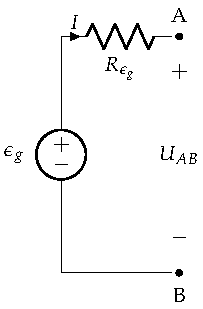
\includegraphics[height=0.43\textheight]{../figs/FuenteTensionRealDC.pdf}
        \end{center}
    
        \begin{center}
        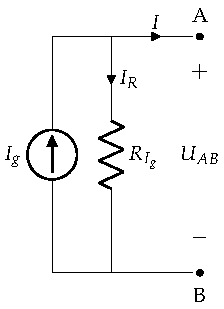
\includegraphics[height=0.43\textheight]{../figs/FuenteCorrienteRealDC.pdf}
        \end{center}
    \end{column}
    
    \begin{column}{0.75\columnwidth}
        La salida de tensión de una fuente de tensión es:
        \[
          U_{AB} = \epsilon_g - R_{\epsilon_g} \cdot I
        \]
        Y de una fuente de corriente:
        \[
          I = I_g - \frac{U_{AB}}{R_{I_g}} \quad \rightarrow \quad U_{AB} = R_{I_g} \cdot I_g - R_{I_g} \cdot I
        \]
        Las \alert{fuentes son equivalentes cuando} las ecuaciones coinciden para cualquier combinación \((U_{AB}, I)\):
        \[
            \boxed{R_g = R_{\epsilon_g} = R_{I_g}} \;\; \textrm{\footnotesize{(resultado de la diapositiva anterior)}}
        \]
        \[
          \boxed{\epsilon_g = R_g \cdot I_g} \Leftrightarrow \boxed{I_g = \frac{\epsilon_g}{R_g}}
        \]
    \end{column}
    \end{columns}
\end{frame}

%%%%%%%%%%%%%%%%

\begin{frame}{Generadores dependientes} \label{diapo:fuentes_dependientes}
    No tienen valores de $\epsilon_g$ o $I_g$ fijos, sino que estos \alert{dependen de la tensión o corriente en otros puntos de la red}:
	\begin{center}
		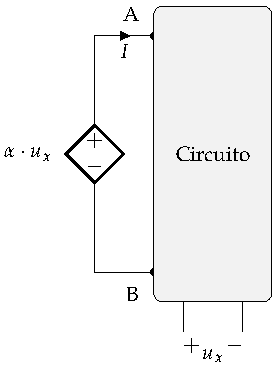
\includegraphics[height=4.6cm]{../figs/FuenteTensionDependienteTension.pdf}\label{fig.tension-tension}\hfill
		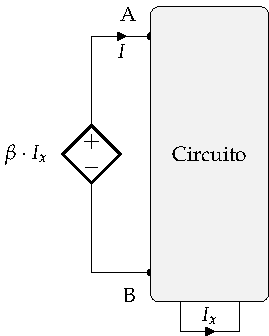
\includegraphics[height=4.6cm]{../figs/FuenteTensionDependienteCorriente.pdf}\label{fig.tension-corriente}\hfill
		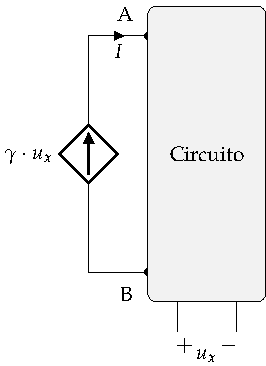
\includegraphics[height=4.6cm]{../figs/FuenteCorrienteDependienteTension.pdf}\label{fig.corriente-tension}\hfill
		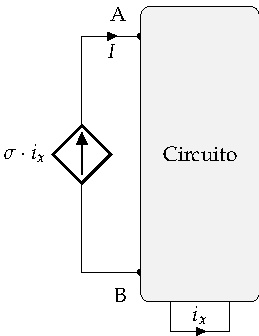
\includegraphics[height=4.6cm]{../figs/FuenteCorrienteDependienteCorriente.pdf}\label{fig.corriente-corriente}
	\end{center}
\end{frame}

%%%%%%%%%%%%%%%%

%\begin{frame}{Otros receptores}
%    \begin{itemize}
%        \item Compuestos por combinaciones de los elementos básicos
%        \item Se caracterizan por su \alert{fuerza contraelectromotriz} (f.c.e.m, E' o $\varepsilon'$): energía por unidad de carga que transforman en otro tipo (no calor)
%    \end{itemize}
%    \begin{columns}
%    \begin{column}{0.3\columnwidth}
%    \begin{center}
%    \includegraphics[height=0.4\textheight]{../figs/receptor_ideal.pdf}
%    
%    \alert{Ideal}
%    \begin{equation*}
%        u_{AB}=\epsilon'
%    \end{equation*}
%    \end{center}
%    \end{column}
%    \begin{column}{0.3\columnwidth}
%    \begin{center}
%    \includegraphics[height=0.4\textheight]{../figs/receptor_real.pdf}
%    
%    \alert{Real} (pérdidas)
%    \begin{equation*}
%        u_{AB}>\epsilon'
%    \end{equation*}
%    \end{center}
%    \end{column}
%    \begin{column}{0.4\columnwidth}
%    \begin{align*}
%        P_u&=\epsilon'\cdot I\\
%        P_p&=R_{\epsilon'}\cdot I^2\\
%        P_a&=U_{AB}\cdot I\\
%        \Aboxed{U_{AB}&=\epsilon'+R_{\epsilon'}\cdot I}
%    \end{align*}
%    \end{column}
%    \end{columns}
%\end{frame}

%%%%%%%%%%%%%%%%

\begin{frame}{Eficiencia}
    
    Cociente entre la potencia de salida y la potencia de entrada:
    \begin{itemize}
        \item \alert{Receptor} (generalmente, motor):
    \begin{equation*}
      \eta_m = \frac{P_{\textrm{útil}}}{P_{\textrm{absorbida}}}
    \end{equation*}
    
    \item \alert{Generador}:
    \begin{equation*}
      \eta_g = \frac{P_{\textrm{entregada}}}{P_{\textrm{producida}}}
    \end{equation*}
    \end{itemize}

    \vspace{4mm}
    \alert{Cualquier máquina tiene pérdidas} (por disipación de energía en forma de calor):
    
    \begin{equation*}
      \boxed{\eta < 1}
    \end{equation*}
\end{frame}

%%%%%%%%%%%%%%%%

\begin{frame}{Balance de potencias}
    \begin{itemize}
        \item Ejemplo: \alert{motor}

        \vspace{1mm}
        Caracterizado por su \alert{fuerza contraelectromotriz} (f.c.e.m., $\epsilon'$): energía por unidad de carga, que transforma en otro tipo de energía (mecánica, química, etc.)
    \end{itemize}
    \begin{columns}
    \begin{column}{0.3\columnwidth}
        \begin{center}
        \includegraphics[height=0.5\textheight]{../figs/receptor_real.pdf}
        
        \alert{Real} (con pérdidas)
        \begin{equation*}
            U_{AB}>\epsilon'
        \end{equation*}
        \end{center}
    \end{column}
    \begin{column}{0.4\columnwidth}
    \vspace{-4mm}
    \begin{align*}
        \Aboxed{ P_{\textrm{útil}} &= P_{\textrm{absorbida}} - P_{\textrm{pérdidas}} }\\[7pt]
        P_{\textrm{útil}} &= \epsilon'\cdot I\\[7pt]
        P_{\textrm{pérdidas}} &= R_{\epsilon'}\cdot I^2 \;\; \text{\small{(ley de Joule)}}\\[7pt]
        P_{\textrm{absorbida}} &= U_{AB}\cdot I\\[15pt]
        & \hspace{-25mm}\text{Dado que } U_{AB}>\epsilon', \;\eta_m < 1:\\[7pt]
        \eta_m &= \frac{P_{\textrm{útil}}}{P_{\textrm{absorbida}}} = \frac{\epsilon' \cdot \bcancel{I}}{U_{AB} \cdot \bcancel{I}} < 1
    \end{align*}
    \end{column}
    \end{columns}
\end{frame}

%%%%%%%%%%%%%%%%

\section{Leyes de Kirchhoff}

\begin{frame}{Definiciones} \label{definiciones_mallas}
    \begin{description}
        \item[{Nudo}] \hspace{2mm}unión de \alert{3} o más conductores \hspace{3mm}(en la figura, los puntos A, B, C y D)
        \item[{Rama}] \hspace{2mm}elementos conectados entre dos nudos consecutivos 
        
        \hspace{2mm}(A-B, A-C, A-D, B-C, B-D y C-D)
        \item[{Lazo}] \hspace{2mm}conjunto de ramas que forman un camino cerrado
        
        \hspace{2mm}(ACDA, ACBDA, ACDBA, ABCDA, ABCA, ABDA, BCDB)
        \item[{Malla}] \hspace{2mm}lazo que no contiene ningún otro en su interior 
        \hspace{3mm}(ABCA, ABDA, BCDB)
    \end{description}

    \begin{center}
        \includegraphics[height=0.5\textheight]{../figs/mallas.pdf}
    \end{center}
\end{frame}

%%%%%%%%%%%%%%%%

\begin{frame}{Primera Ley de Kirchhoff (1LK)}
    \begin{itemize}
        \item La \alert{1LK} es el principio de \alert{conservación de la carga} aplicado a los circuitos eléctricos:
        \vspace{2mm}
        
        La suma de las corrientes que llegan a un nudo es igual a la suma de las que salen      
    \end{itemize}
    \vspace{2mm}
    \begin{equation*}
            \large{\boxed{\sum_{j=1}^n i_j(t)=0}}
        \end{equation*}
    \begin{center}
        \includegraphics[height=0.4\textheight]{../figs/LKC_FM.pdf}
    \end{center}
    \[
        i_1(t) - i_2(t) + i_3(t) - i_4(t) + i_5(t) = 0
    \]
\end{frame}

%%%%%%%%%%%%%%%%

\begin{frame}{Segunda Ley de Kirchhoff (2LK)}
    \begin{itemize}
        \item La \alert{2LK} es el principio de \alert{conservación de la energía} aplicado a los circuitos:
        \vspace{2mm}
        
        La suma (con signo) de las tensiones a lo largo de un camino cerrado es cero        
    \end{itemize}
    \vspace{2mm}
    \begin{equation*}
            \large{\boxed{\sum_{j=1}^m u_j(t)=0}}
        \end{equation*}
    
    \begin{center}
        \includegraphics[height=0.4\textheight]{../figs/LKV_FM.pdf}
    \end{center}
    \[
        - u_1 (t) - u_2 (t) + u_3(t) + u_4 (t) - u_5 (t)    = 0
    \]

    % La energía producida por un generador es consumida por los receptores del circuito para producir trabajo (mecánico, químico, etc.) o calor.
\end{frame}

%%%%%%%%%%%%%%%%

\begin{frame}{2LK a partir de balance de potencias}
    \begin{itemize}
        \item Ejemplo: \alert{motor} real (con pérdidas)
    \end{itemize}
    \begin{columns}
    \begin{column}{0.3\columnwidth}
        \begin{center}
        \includegraphics[height=0.6\textheight]{../figs/receptor_real.pdf}        
        \end{center}
    \end{column}
    \begin{column}{0.4\columnwidth}
    \begin{align*}
        P_{\textrm{útil}} &= P_{\textrm{absorbida}} - P_{\textrm{pérdidas}}\\[7pt]
        P_{\textrm{útil}} &= \epsilon'\cdot I\\[7pt]
        P_{\textrm{pérdidas}} &= R_{\epsilon'}\cdot I^2 \;\; \text{\small{(ley de Joule)}}\\[7pt]
        P_{\textrm{absorbida}} &= U_{AB}\cdot I\\[15pt]
        & \hspace{-25mm}\text{Dividiendo en ambos lados por } I, \text{ se obtiene 2LK:}\\[7pt]
        \Aboxed{U_{AB}&=\epsilon'+R_{\epsilon'}\cdot I}
    \end{align*}
    \end{column}
    \end{columns}
\end{frame}

%%%%%%%%%%%%%%%%

\begin{frame}{Ejercicio}
    \vspace{5mm}
    Un generador cuya \textit{fem} es de \qty{120}{\volt} y resistencia de \qty{0.2}{\ohm}, da una corriente de \qty{20}{\ampere} a un motor situado a \qty{300}{\meter} de distancia y de resistencia \qty{0.5}{\ohm}. 
    
    La línea que los conecta es de cobre, de resistividad \qty{17.24}{\milli\ohm\milli\meter\squared\per\meter}. 
    
    Sabiendo que el motor absorbe \qty{10.2}{\kWh} en \qty{5}{\hour}, se debe hallar:
    \vspace{3mm}
    
    \begin{enumerate}
        \item La fuerza contraelectromotriz (\textit{fcem}) del motor
        \item La sección de los conductores de la línea
        \item Los rendimientos de: motor, generador, línea y rendimiento total
        \item El balance general de potencias
    \end{enumerate}
    \vspace{5mm}
    \alert{Solución}: \href{https://raw.githubusercontent.com/ETSIDI-IE/tc/master/docs/ejercicios_clase/TC1_01_Ejercicio_clase_LBB.pdf}{aquí}
\end{frame}

%%%%%%%%%%%%%%%%

\begin{frame}{Ejercicio}
    \vspace{5mm}
    Un generador de corriente continua alimenta dos cargas. La primera de estas cargas está situada a \qty{2100}{\meter} del generador, tiene una resistencia de \qty{215}{\ohm} y rendimiento unidad. La segunda carga está situada \qty{270}{\meter} después de la primera, tiene una potencia de \qty{4662}{\watt}, un rendimiento del 75\% y una tensión aplicada de \qty{420}{\volt}.

    La línea es de cobre, de \qty{6}{\milli\meter\squared} de sección y con una resistividad de \qty{17.24}{\milli\ohm\milli\meter\squared\per\meter}.
    
    \vspace{4mm}
    
    Con esta información, se debe calcular:
    
    \vspace{1mm}
    
    \begin{enumerate}
        \item La tensión en bornes del generador
        \item La corriente entregada por el generador
        \item El rendimiento de la instalación
    \end{enumerate}
    \vspace{5mm}
    \alert{Solución}: \href{https://raw.githubusercontent.com/ETSIDI-IE/tc/master/docs/ejercicios_clase/TC1_01_Ejercicio_clase2_LBB.pdf}{aquí}
\end{frame}

%%%%%%%%%%%%%%%%

\subsection{Asociación de elementos}

\begin{frame}{Asociación de elementos}
    Las principales formas de asociar elementos en un circuito son:
    \vspace{3mm}
    \begin{itemize}
        \item \alert{Serie}: \textit{final}  de un elemento conectado con \textit{principio} del siguiente $\rightarrow$ \alert{misma corriente}
        \vspace{3mm}
        \item \alert{Paralelo}: todos los principios conectados en un punto, todos los finales en otro $\rightarrow$ 
        
        \hspace{15.5mm} \alert{misma diferencia de potencial}
        \vspace{3mm}
        \item \alert{Mixto}: combinación de serie y paralelo
        \vspace{3mm}
        \item \alert{Estrella - Triángulo}: conexión de cargas trifásicas
    \end{itemize}    
\end{frame}

%%%%%%%%%%%%%%%%

\begin{frame}{Conexión en serie}
    \begin{columns}
    \begin{column}{0.3\columnwidth}
        \begin{center}
        \includegraphics[height=0.85\textheight]{../figs/AsociacionSerie.pdf}
        \end{center}
    \end{column}
    \begin{column}{0.7\columnwidth}
        Un conjunto de elementos están asociados en serie cuando circula la \alert{misma corriente} por todos ellos:
        \begin{align*}      
          u_1(t) &= R_1 \cdot i(t)\\
          u_2(t) &= R_2 \cdot i(t)\\
          u_3(t) &= R_3 \cdot i(t)      
        \end{align*}    
        Aplicando \alert{2LK}:
        \begin{align*} 
            u(t) &= u_1(t) + u_2(t) + u_3(t) \\
            u(t) &= i(t) \cdot (R_1 + R_2 + R_3)
        \end{align*}    
    
        Definimos la \alert{resistencia equivalente} de la conexión serie:
        \[
          \boxed{R_{eq} = \sum_{i = 1}^n R_i} \quad \textrm{dado que} \;\; u(t) = R_{eq} \cdot i(t)
        \]
    \end{column}
    \end{columns}
\end{frame}

%%%%%%%%%%%%%%%%

\begin{frame}{Conexión en serie: \hspace{2mm}divisor de tensión}
    \begin{columns}
    \begin{column}{0.3\columnwidth}
        \begin{center}
            \includegraphics[height=0.85\textheight]{../figs/AsociacionSerie.pdf}
        \end{center}
    \end{column}
    \begin{column}{0.7\columnwidth}
        \vspace{2mm}
    
        De las ecuaciones anteriores tenemos:
        \vspace{-2mm}
        \begin{align*}
          i(t) &= \frac{u(t)}{R_1 + R_2 + R_3}\\
          u_3(t) &= R_3 \cdot i(t)
        \end{align*}        
        Por tanto, la \alert{tensión parcial} \(u_3(t)\) se puede expresar en función de la tensión total \(u(t)\): 
        \vspace{-2mm}
        \begin{equation*}
          u_3(t) = u(t) \cdot \frac{R_3}{R_1 + R_2 + R_3}  
        \end{equation*}
        
        \alert{En general}, para cualquiera de las resistencias, $R_i$:
        \begin{equation*}
          \boxed{u_i(t) = u(t) \cdot \frac{R_i}{R_{eq}}}
        \end{equation*}
        \centering \small{(expresión útil para agilizar la resolución de algunos ejercicios)}
    \end{column}
    \end{columns}
\end{frame}

%%%%%%%%%%%%%%%%

\begin{frame}{Conexión en serie de bobinas} \label{diapo:bobinas_serie}
    \begin{columns}
    \begin{column}{0.3\columnwidth}
    \begin{center}
    \includegraphics[height=0.85\textheight]{../figs/BobinasSerie.pdf}
    \end{center}
    \end{column}
    \begin{column}{0.7\columnwidth}
    Mismos pasos que en el caso de las resistencias:
    \begin{align*}
      u(t) & = u_1(t) + u_2(t) + u_3(t)\\
      u_1(t) &= L_1 \cdot \frac{di(t)}{dt}\\
      u_2(t) &= L_2 \cdot \frac{di(t)}{dt}\\
      u_3(t) &= L_3 \cdot \frac{di(t)}{dt}\\
      u(t)& = \frac{di(t)}{dt} \cdot (L_1 + L_2 + L_3)\\
      \Aboxed{L_{eq} &= \sum_{i = 1}^n L_i} \quad \textrm{dado que} \;\; u(t) = L_{eq} \cdot \frac{di(t)}{dt}
    \end{align*}
    \end{column}
    \end{columns}
\end{frame}

%%%%%%%%%%%%%%%%

\begin{frame}{Conexión en serie de condensadores}
    \begin{columns}
    \begin{column}{0.3\columnwidth}
    \begin{center}
    \includegraphics[height=0.85\textheight]{../figs/CondensadoresSerie.pdf}
    \end{center}
    \end{column}
    \begin{column}{0.7\columnwidth}
    \begin{align*}
      u(t) & = u_1(t) + u_2(t) + u_3(t)\\
      i(t) &= C_1 \cdot \frac{du_1(t)}{dt}= C_2 \cdot \frac{du_2(t)}{dt}= C_3 \cdot \frac{du_3(t)}{dt}\\
      u_1(t)&=\dfrac{1}{C_1}\cdot\int_{0}^{t} i(\tau)\, d\tau\\
      u_2(t)&=\dfrac{1}{C_2}\cdot\int_{0}^{t} i(\tau)\, d\tau\\
      u_3(t)&=\dfrac{1}{C_3}\cdot\int_{0}^{t} i(\tau)\, d\tau\\
      u(t)& = \int_{0}^{t} i(\tau)\,d\tau \cdot \left(\dfrac{1}{C_1}+\dfrac{1}{C_2}+\dfrac{1}{C_3}\right)\\
      \Aboxed{\frac{1}{C_{eq}} &= \sum_{i = 1}^n \frac{1}{C_i}} \quad \textrm{dado que} \;\; i(t) = C_{eq} \cdot \frac{du(t)}{dt}
    \end{align*}
    \end{column}
    \end{columns}
    \hyperlink{diapo:condensadores_paralelo}{.}
\end{frame}

%%%%%%%%%%%%%%%%

\begin{frame}{Conexión en serie de generadores}
    \begin{block}{Generadores de tensión}
    \begin{itemize}
    \item Pueden conectarse en serie \alert{sin restricción} (tanto generadores ideales como reales)

    \vspace{-5mm}
    \begin{align*}
      \epsilon_T &= \sum_{i = 1}^N \epsilon_i\\
      R_{\epsilon_T} &= \sum_{i = 1}^N R_{\epsilon_i}
    \end{align*}
    \end{itemize}
    \vspace{-3mm}
    \end{block}
    
    \begin{block}{Generadores de corriente}
    \begin{itemize}
    \vspace{2mm}
    \item \alert{Ideal}: todas las fuentes \alert{deben ser idénticas} (valor y sentido)
    \vspace{2mm}
    \item \alert{Real}:  sin restricción 
        \begin{itemize}
        \item \normalsize{Transformación a fuentes de tensión para obtener la \alert{fuente equivalente}}
        \end{itemize}
    \end{itemize}
    \end{block}
\end{frame}

%%%%%%%%%%%%%%%%

\begin{frame}{Ejemplo: \hspace{3mm}fuentes de corriente reales en serie}

    \vspace{2mm}
    Se \hyperlink{diapo:transformacion_fuentes}{transforman} primero cada una de las fuentes de corriente en fuentes de tensión:
    % Sobre la cross-reference usando "hyperlink": https://tex.stackexchange.com/questions/70143/cross-reference-with-custom-text

    \vspace{1mm}
    \begin{minipage}[c]{0.05\linewidth}
        \hfill
    \end{minipage}
    \begin{minipage}[c]{0.15\linewidth}
        \begin{center}
        \includegraphics[height=0.8\textheight]{../figs/FuentesCorrienteReales_serie.pdf}
        \end{center}
    \end{minipage}
    \begin{minipage}[c]{0.08\linewidth}
        \begin{center}
        $\LARGE \xrightarrow{\hspace*{0.5cm}}$ % https://latex.org/forum/viewtopic.php?t=3894
        \end{center}
    \end{minipage}
    \begin{minipage}[c]{0.15\linewidth}
        \begin{center}
        \includegraphics[height=0.8\textheight]{../figs/FuentesTensionReales_serie.pdf}
        \end{center}
    \end{minipage}
    \begin{minipage}[c]{0.05\linewidth}
        \hfill
    \end{minipage}
    \begin{minipage}[c]{0.45\linewidth}
        Donde:
        \[
          \epsilon_1 = I_{g_1} \cdot R_{I_{g_1}}
        \]  
        \[
          \epsilon_2 = I_{g_2} \cdot R_{I_{g_2}}
        \] 
          
        \[
          R_{\epsilon_1} = R_{I_{g_1}}
        \]
        \[
          R_{\epsilon_2} = R_{I_{g_2}}
        \]

        \vspace{6mm}
        \centering \small{(continúa en la siguiente diapositiva)}
    \end{minipage}
\end{frame}

%%%%%%%%%%%%%%%%

\begin{frame}{Ejemplo: \hspace{3mm}fuentes de corriente reales en serie \hspace{3mm}(continuación)}

    \vspace{1mm}
    Las fuentes de tensión en serie se transforman directamente en una fuente equivalente, y esta se transforma de vuelta en una fuente de corriente:

    %\vspace{4mm}
    \begin{minipage}[c]{0.15\linewidth}
        \begin{center}
        \includegraphics[height=0.45\textheight]{../figs/FuenteTensionReal_totalSerie.pdf}
        \end{center}
    \end{minipage}
    \begin{minipage}[c]{0.08\linewidth}
        $\LARGE \xrightarrow{\hspace*{0.5cm}}$ % https://latex.org/forum/viewtopic.php?t=3894
    \end{minipage}
    \begin{minipage}[c]{0.15\linewidth}
        \begin{center}
        \includegraphics[height=0.45\textheight]{../figs/FuenteCorrienteReal_totalSerie.pdf}
        \end{center}
    \end{minipage}
    \begin{minipage}[c]{0.08\linewidth}
        \hfill
    \end{minipage}
    \begin{minipage}[c]{0.47\linewidth}
        \vspace{4mm}
        Donde:
        \[
          \epsilon_T = \epsilon_1 + \epsilon_2 = I_{g_1} \cdot R_{I_{g_1}} + I_{g_2} \cdot R_{I_{g_2}}
        \]  
        \[
          R_{\epsilon_T} = R_{\epsilon_1} + R_{\epsilon_2} = R_{I_{g_1}} + R_{I_{g_2}}
        \] 

        \vspace{2mm}
        Y finalmente:
        \[
          \boxed{
          I_{g_T} = \frac{\epsilon_T}{R_{I_{g_T}}} = \frac{I_{g_1} \cdot R_{I_{g_1}} + I_{g_2} \cdot R_{I_{g_2}}}{R_{I_{g_1}} + R_{I_{g_2}}}
          }
        \]
        \[
          \boxed{
          R_{I_{g_T}} = R_{\epsilon_T} = R_{I_{g_1}} + R_{I_{g_2}}
          }
        \]
    \end{minipage}
\end{frame}

%%%%%%%%%%%%%%%%

\begin{frame}{Conexión en paralelo}
    \begin{columns}
    \begin{column}{0.4\columnwidth}
        \vspace{-10mm}
        \begin{center}
        \includegraphics[width=1\linewidth]{../figs/AsociacionParalelo.pdf}
        \end{center}
    \end{column}
    \begin{column}{0.6\columnwidth}
        Un conjunto de elementos están asociados en paralelo cuando están sometidos a la \alert{misma tensión}:
        \vspace{-2mm}
        \begin{align*}      
          i_1(t) &= u(t)/R_1\\
          i_2(t) &= u(t)/R_2\\
          i_3(t) &= u(t)/R_3      
        \end{align*}    
        \vspace{-2mm}
        Aplicando \alert{1LK}:
        \begin{align*} 
            i(t)& = i_1(t) + i_2(t) + i_3(t) \\
            i(t) &= u(t) \cdot \left(\frac{1}{R_1} + \frac{1}{R_2} + \frac{1}{R_3}\right)
        \end{align*}    
    
        Definimos la \alert{resistencia equivalente} del paralelo:
        \[
          \boxed{\frac{1}{R_{eq}} = \sum_{i = 1}^n \frac{1}{R_i}} \quad \textrm{dado que} \;\; u(t) = R_{eq} \cdot i(t)
        \]
    \end{column}
    \end{columns}
\end{frame}

%%%%%%%%%%%%%%%%

\begin{frame}{Conexión en paralelo: \hspace{3mm} caso particular de dos resistencias}  \label{diapo:2R_paralelo}

    \vspace{5mm}
    En el caso concreto de \alert{dos resistencias en paralelo}, la expresión es:
    
    \begin{equation*}
      \frac{1}{R_{eq}} = \frac{1}{R_1} + \frac{1}{R_2}
    \end{equation*}
    
    \begin{equation*}
      \boxed{R_{eq} = \frac{R_1 \cdot R_2}{R_1 + R_2}}
    \end{equation*}
    
    \centering \small{(conveniente recordarla para agilizar la resolución de algunos ejercicios)}

    \vspace{2mm}
    
    \noindent\rule{\textwidth}{0.5pt}

    \vspace{2mm}

    Para `$N$' \alert{resistencias iguales} asociadas en paralelo, cada una de valor `$R$': 
    \[
        R_{eq} = \frac{R}{N}
    \]
\end{frame}

%%%%%%%%%%%%%%%%

\begin{frame}{Conductancia}

    \vspace{4mm}
    Para \alert{simplificar las operaciones} en conexiones en paralelo, es conveniente utilizar el inverso de la resistencia, la \alert{conductancia} $G$:
    \vspace{2mm}
    \begin{equation*}
      G = \frac{1}{R}
    \end{equation*}
    
    Así, en lugar de\ldots{}
    \vspace{-2mm}
    \begin{align*}
      \frac{1}{R_{eq}} &= \sum_{i = 1}^n \frac{1}{R_i}\\[7pt]
      u(t) &= R_{eq} \cdot i(t)
    \end{align*}
    \ldots{}se puede escribir:
    \begin{equation*}
      \hspace{43mm} \boxed{G_{eq} = \sum_{i = 1}^n G_i} \quad \textrm{y usar} \;\; \underbrace{i(t) = G_{eq} \cdot u(t)}_{\text{ley de Ohm}}
    \end{equation*}
\end{frame}

%%%%%%%%%%%%%%%%

\begin{frame}{Conexión en paralelo: \hspace{2mm} divisor de corriente}
    \begin{columns}
    \begin{column}{0.4\columnwidth}
        \vspace{-10mm}
        \begin{center}
        \includegraphics[width=1\linewidth]{../figs/AsociacionParalelo.pdf}
        \end{center}
    \end{column}
    \begin{column}{0.6\columnwidth}
    
        \vspace{2mm}
        De las ecuaciones anteriores tenemos:
        
        \begin{equation*}
          u(t) = \frac{i(t)}{G_1 + G_2 + G_3} \qquad
          i_3(t) = G_3 \cdot u(t)
        \end{equation*}
        
        Por tanto, la \alert{corriente parcial} \(i_3(t)\) se puede expresar en función de la corriente total \(i(t)\): 
        \begin{equation*}
          i_3(t) = i(t) \cdot \frac{G_3}{G_1 + G_2 + G_3}  
        \end{equation*}
        
        \alert{En general}, para cualquiera de las conductancias, $G_j$:
        \begin{equation*}
          \boxed{i_j(t) = i(t) \cdot \frac{G_j}{G_{eq}} = i(t) \cdot \frac{R_{eq}}{R_j}}
        \end{equation*}

        \vspace{-1mm}
        \centering \small{(expresión útil para agilizar la resolución de ejercicios)}
    \end{column}
    \end{columns}    
\end{frame}

%%%%%%%%%%%%%%%%

\begin{frame}{Divisor de corriente: \hspace{3mm} caso particular de dos resistencias}

    \vspace{5mm}
    En el caso concreto de \alert{dos resistencias en paralelo}, la expresión es:
    
    \begin{equation*}
      i_1(t) = i(t) \cdot \frac{G_1}{G_1 + G_2} = i(t) \cdot \frac{\hyperlink{diapo:2R_paralelo}{R_1 \parallel R_2}}{R_1} = i(t) \cdot \frac{\cancel{R_1} \cdot R_2}{R_1 + R_2} \cdot \frac{1}{\cancel{R_1}}
    \end{equation*} % Sobre la cross-reference usando "hyperlink": https://tex.stackexchange.com/questions/70143/cross-reference-with-custom-text
    
    \begin{equation*}
      \boxed{i_1(t) = i(t) \cdot \frac{R_2}{R_1 + R_2}}
    \end{equation*}
    
    \centering \small{(conveniente recordarla para agilizar la resolución de algunos ejercicios)} 

    \vspace{2mm}
    
    \noindent\rule{\textwidth}{0.5pt}

    \vspace{2mm}

    Para `$N$' \alert{resistencias iguales} asociadas en paralelo: 
    \[
        i_j(t) = \frac{i(t)}{N}
    \]
\end{frame}

%%%%%%%%%%%%%%%%

\begin{frame}{Conexión en paralelo de condensadores} \label{diapo:condensadores_paralelo}
    \begin{columns}
    \begin{column}{0.4\columnwidth}
        \vspace{-10mm}
        \begin{center}
        \includegraphics[width=1.05\linewidth]{../figs/CondensadoresParalelo.pdf}
        \end{center}
    \end{column}
    \begin{column}{0.6\columnwidth}
    
    \vspace{2mm}
    Mismos pasos que en el caso de las resistencias:

    \vspace{-5mm}
    \begin{align*}
      i(t) & = i_1(t) + i_2(t) + i_3(t)\\
      i_1(t) &= C_1 \cdot \frac{du(t)}{dt}\\
      i_2(t) &= C_2 \cdot \frac{du(t)}{dt}\\
      i_3(t) &= C_3 \cdot \frac{du(t)}{dt}\\
      i(t)& = \frac{du(t)}{dt} \cdot (C_1 + C_2 + C_3)\\
      \Aboxed{C_{eq} &= \sum_{i = 1}^n C_i} \quad \textrm{dado que} \;\; i(t) = C_{eq} \cdot \frac{du(t)}{dt}
    \end{align*}
    \end{column}
    \end{columns}      
\end{frame}

%%%%%%%%%%%%%%%%

\begin{frame}{Conexión en paralelo de bobinas}
    \vspace{2mm}
    \begin{columns}
    \begin{column}{0.4\columnwidth}
        \vspace{-10mm}
        \begin{center}
        \includegraphics[width=1\linewidth]{../figs/BobinasParalelo.pdf}
        \end{center}
    \end{column}
    \begin{column}{0.6\columnwidth}
    \begin{align*}
      i(t)& = i_1(t) + i_2(t) + i_3(t)\\
      u(t) &= L_1 \cdot \frac{di_1(t)}{dt}= L_2 \cdot \frac{di_2(t)}{dt}= L_3 \cdot \frac{di_3(t)}{dt}\\
      i_1(t)&=\dfrac{1}{L_1}\cdot\int_{0}^{t} u(\tau)\, d\tau\\
      i_2(t)&=\dfrac{1}{L_2}\cdot\int_{0}^{t} u(\tau)\, d\tau\\
      i_3(t)&=\dfrac{1}{L_3}\cdot\int_{0}^{t} u(\tau)\, d\tau\\
      i(t)& = \int_{0}^{t} u(\tau)\,d\tau \cdot \left(\dfrac{1}{L_1}+\dfrac{1}{L_2}+\dfrac{1}{L_3}\right)\\
      \Aboxed{\frac{1}{L_{eq}} &= \sum_{i = 1}^n \frac{1}{L_i}} \quad \textrm{dado que} \;\; u(t) = L_{eq} \cdot \frac{di(t)}{dt}
    \end{align*}
    \end{column}
    \end{columns}
    \hyperlink{diapo:Teoremas}{.}
\end{frame}

%%%%%%%%%%%%%%%%

\begin{frame}{Conexión en paralelo de generadores}

    \begin{block}{Generadores de tensión}
    \begin{itemize}
    \vspace{2mm}
    \item \alert{Ideal}: todas las fuentes \alert{deben ser idénticas} (valor y polaridad)
    \vspace{2mm}
    \item \alert{Real}:  sin restricción
        \begin{itemize}
        \item \normalsize{Transformación a fuentes de corriente para obtener la \alert{fuente equivalente}}
        \end{itemize}
    \end{itemize}
    \end{block}    
    
    \begin{block}{Generadores de corriente}
    \begin{itemize}
    \item Pueden conectarse en paralelo \alert{sin restricción}

    \vspace{-5mm}
    \begin{align*}
      I_{g_T} &= \sum_{i = 1}^N I_{g_i}\\
      G_{g_T} &= \sum_{i = 1}^N G_{g_i}
    \end{align*}
    \end{itemize}
    \vspace{-3mm}
    \end{block}
\end{frame}

%%%%%%%%%%%%%%%%

\begin{frame}{Ejemplo: \hspace{3mm}fuentes de tensión reales en paralelo}

    \vspace{2mm}
    Se \hyperlink{diapo:transformacion_fuentes}{transforman} primero cada una de las fuentes de tensión en fuentes de corriente:
    % Sobre la cross-reference usando "hyperlink": https://tex.stackexchange.com/questions/70143/cross-reference-with-custom-text

    \vspace{2mm}
    \begin{minipage}[c]{0.38\linewidth}
        \begin{center}
        \includegraphics[height=0.45\textheight]{../figs/FuentesTensionReales_paralelo.pdf}
        \end{center}
    \end{minipage}
    \begin{minipage}[c]{0.08\linewidth}
        \begin{center}
        $\LARGE \xrightarrow{\hspace*{0.5cm}}$ % https://latex.org/forum/viewtopic.php?t=3894
        \end{center}
    \end{minipage}
    \begin{minipage}[c]{0.4\linewidth}
        \begin{center}
        \includegraphics[height=0.45\textheight]{../figs/FuentesCorrienteReales_paralelo.pdf}
        \end{center}
    \end{minipage}

    \vspace{4mm}
    
    Donde:
    \[
      I_{g_1} = \frac{\epsilon_1}{R_{\epsilon_1}} \qquad I_{g_2} = \frac{\epsilon_2}{R_{\epsilon_2}} \qquad R_{I_{g_1}} = R_{\epsilon_1} \qquad R_{I_{g_2}} = R_{\epsilon_2}
    \]

    \vspace{2mm}
    \centering \small{(continúa en la siguiente diapositiva)}
\end{frame}

%%%%%%%%%%%%%%%%

\begin{frame}{Ejemplo: \hspace{3mm}fuentes de tensión reales en paralelo \hspace{3mm}(continuación)}

    \vspace{2mm}
    Las fuentes de corriente en paralelo se transforman directamente en una fuente equivalente, y esta se transforma de vuelta en una fuente de tensión:

    \begin{minipage}[c]{0.45\linewidth}
        \begin{center}
        \includegraphics[height=0.45\textheight]{../figs/FuenteCorrienteReal_total.pdf}
        \end{center}
    \end{minipage}
    \begin{minipage}[c]{0.08\linewidth}        
        $\LARGE \xrightarrow{\hspace*{0.5cm}}$        
    \end{minipage}
    \begin{minipage}[c]{0.3\linewidth}
        \begin{center}
        \includegraphics[height=0.45\textheight]{../figs/FuenteTensionReal_total.pdf}
        \end{center}
    \end{minipage}

    \vspace{-2mm}
    \begin{minipage}[c]{0.45\linewidth}
        \begin{center}
            \begin{align*}
            I_{g_T} &= I_{g_1} + I_{g_2} = \frac{\epsilon_1}{R_{\epsilon_1}} + \frac{\epsilon_2}{R_{\epsilon_2}} \\[2pt]
            R_{I_{g_T}} &= R_{I_{g_1}} \parallel R_{I_{g_2}} = R_{\epsilon_1} \parallel R_{\epsilon_2}
            \end{align*}
        \end{center}
    \end{minipage}
    \begin{minipage}[c]{0.08\linewidth}  
        \hfill
    \end{minipage}
    \begin{minipage}[c]{0.3\linewidth}
        \[
            \boxed{ \epsilon_T = R_{\epsilon_T} \cdot I_{g_T} =  \frac{\epsilon_1 \cdot R_{\epsilon_2} + \epsilon_2 \cdot R_{\epsilon_1}}{R_{\epsilon_1} + R_{\epsilon_2}}}
            % Paso intermedio despues de "R_{\epsilon_T} \cdot I_{g_T}":
            % R_{\epsilon_T} \cdot \left( \frac{\epsilon_1}{R_{\epsilon_1}} + \frac{\epsilon_2}{R_{\epsilon_2}
        \]
        \vspace{-3mm}
        \[
            \boxed{ R_{\epsilon_T} = R_{I_{g_T}} = R_{\epsilon_1} \parallel R_{\epsilon_2} }
        \]
    \end{minipage}
\end{frame}

%%%%%%%%%%%%%%%%

\begin{frame}{Interludio: \hspace{3mm}aplicaciones del efecto Joule}
    \vspace{1mm}
    La empresa Manitoba Hydro, en Canadá, usa picos de corriente controlados para deshielo de líneas de transmisión eléctrica (\alert{clica en la imagen}):
		\begin{figure}[H]
			\centering
			\href{https://twitter.com/manitobahydro/status/1616529065879666688?t=zpgrdypQRYD2SJVQbOHkeg&s=19}{\includegraphics[width=.39\linewidth]{../figs/Joule_Manitoba.png}}
		\end{figure}
\end{frame}

%%%%%%%%%%%%%%%%

\begin{frame}{Conexión mixta}{Ejemplo}
    \vspace{5mm}
    Calcular la corriente que aporta la fuente de tensión del siguiente circuito:
		\begin{figure}[H]
			\centering
			\includegraphics{../figs/ej1_BT1.pdf}
		\end{figure}
    \vspace{5mm}
    \alert{Solución}: \qty{6.04}{\ampere}
\end{frame}

%%%%%%%%%%%%%%%%

\begin{frame}{Conexión estrella - triángulo}
    \begin{columns}
    \begin{column}{0.5\columnwidth}
    \begin{center}
    \includegraphics[width=.9\linewidth]{../figs/Conexion_Triangulo.pdf}
    \end{center}
    \end{column}
    \begin{column}{0.5\columnwidth}
    \begin{center}
    \includegraphics[width=.9\linewidth]{../figs/Conexion_Estrella.pdf}
    \end{center}
    \end{column}
    \end{columns}
\end{frame}

%%%%%%%%%%%%%%%%

\begin{frame}{Conexión estrella - triángulo} 

    \vspace{2mm}
    Existen acomplamientos que no se simplifican mediante reducciones ``serie'' o ``paralelo''
    
    \vspace{1mm}
    Son necesarias \alert{otras transformaciones}:
    
    \vspace{-2mm}
    \begin{center}              
        \includegraphics[width=.9\linewidth]{../figs/estrella_a_triangulo.pdf}
    \end{center}    
\end{frame}

%%%%%%%%%%%%%%%%

\begin{frame}
{Conexión triángulo}
    \begin{columns}
    \begin{column}{0.4\columnwidth}
    \begin{center}
    \includegraphics[width=1.1\linewidth]{../figs/Conexion_Triangulo.pdf}
    \end{center}
    \end{column}
    \begin{column}{0.5\columnwidth}
    La resistencia \alert{vista entre los terminales} A y B es la asociación paralelo de $R_{ab}$ con el serie de $R_{bc}$ y $R_{ca}$:
    \begin{equation*}
      R_{AB} = \frac{R_{ab} \cdot (R_{bc} + R_{ca})}{R_{ab} + R_{bc} + R_{ca}}
    \end{equation*}
    % Dado que la equivalencia entre triángulo y estrella tiene que darse en todas las combinaciones de circuito externo posible, podemos centrarnos únicamente en este caso en el que dejamos uno de los terminales "al aire" y calculamos la resistencia vista desde los otros dos. Como veremos, con este caso ya tenemos suficientes ecuaciones para calcular la transformación triángulo-estrella.

    \vspace{3mm}
    De la misma forma, para los terminales B-C y C-A:

    \vspace{-6mm}
    \begin{align*}
      R_{BC} &= \frac{R_{bc} \cdot (R_{ab} + R_{ca})}{R_{ab} + R_{bc} + R_{ca}}\\
      \\
      R_{CA} &= \frac{R_{ca} \cdot (R_{ab} + R_{bc})}{R_{ab} + R_{bc} + R_{ca}}
    \end{align*}
    \end{column}
    \end{columns}
\end{frame}

%%%%%%%%%%%%%%%%

\begin{frame}{Conexión triángulo}
    \begin{columns}
    \begin{column}{0.4\columnwidth}
    \begin{center}
    \includegraphics[width=1.1\linewidth]{../figs/Conexion_Triangulo.pdf}
    \end{center}
    \end{column}
    \begin{column}{0.5\columnwidth}
    Desarrollando los productos:
    \begin{align*}
      R_{AB} &= \frac{R_{ab} \cdot R_{bc}}{R_{ab} + R_{bc} + R_{ca}} + \frac{R_{ab} \cdot R_{ca}}{R_{ab} + R_{bc} + R_{ca}}\\
      \\
      R_{BC} &= \frac{R_{bc} \cdot R_{ab}}{R_{ab} + R_{bc} + R_{ca}} + \frac{R_{bc} \cdot R_{ca}}{R_{ab} + R_{bc} + R_{ca}}\\
      \\
      R_{CA} &= \frac{R_{ca} \cdot R_{ab}}{R_{ab} + R_{bc} + R_{ca}} + \frac{R_{ca} \cdot R_{bc}}{R_{ab} + R_{bc} + R_{ca}}
    \end{align*}
    
    \vspace*{3mm}
    \centering \small{(en un momento veremos para qué 
    
    son útiles estas expresiones)}
    \end{column}
    \end{columns}
\end{frame}

%%%%%%%%%%%%%%%%

\begin{frame}{Conexión estrella}
    \begin{columns}
    \begin{column}{0.4\columnwidth}
    \begin{center}
    \includegraphics[width=1.1\linewidth]{../figs/Conexion_Estrella.pdf}
    \end{center}
    \end{column}
    \begin{column}{0.5\columnwidth}
    La resistencia \alert{vista entre los terminales} A y B es simplemente la asociación serie de $R_{a}$ y $R_{b}$:
    
    \begin{equation*}
        R_{AB} = R_a + R_b
    \end{equation*}    
    \vspace{1mm}
    
    De la misma forma, para los terminales B-C y C-A:  
    \begin{align*}
      R_{BC} &= R_b + R_c\\
      \\
      R_{CA} &= R_c + R_a\\
    \end{align*}
    \end{column}
    \end{columns}
\end{frame}

%%%%%%%%%%%%%%%%

\begin{frame}{Conexión triángulo-estrella: \hspace{3mm}equivalencia}
Combinando las expresiones de las dos diapositivas anteriores:
    \begin{align*}
        \frac{R_{a{\color{red}b}} \cdot R_{{\color{red}b}c}}{R_{ab} + R_{bc} + R_{ca}} + \frac{R_{{\color{blue}a}b} \cdot R_{c{\color{blue}a}}}{R_{ab} + R_{bc} + R_{ca}} &= R_{\color{blue}a} + R_{\color{red}b}\\
        \\
        \frac{R_{a{\color{red}b}} \cdot R_{{\color{red}b}c}}{R_{ab} + R_{bc} + R_{ca}} + \frac{R_{b{\color{green}c}} \cdot R_{{\color{green}c}a}}{R_{ab} + R_{bc} + R_{ca}} &= R_{\color{red}b} + R_{\color{green}c}\\
        \\
        \frac{R_{{\color{blue}a}b} \cdot R_{c{\color{blue}a}}}{R_{ab} + R_{bc} + R_{ca}} + \frac{R_{b{\color{green}c}} \cdot R_{{\color{green}c}a}}{R_{ab} + R_{bc} + R_{ca}} &= R_{\color{green}c} + R_{\color{blue}a}
    \end{align*}
    
    Para \alert{convertir de triángulo a estrella}: la expresión, por ejemplo, para $R_a$, se obtiene combinando la primera ecuación, menos la segunda, más la tercera (siguiente diapositiva)
\end{frame}

%%%%%%%%%%%%%%%%

\begin{frame}{Conversión de triángulo a estrella}
    \begin{columns}
    \begin{column}{0.3\columnwidth}
    \begin{center}
    \includegraphics[width=.9\linewidth]{../figs/Conexion_Triangulo.pdf}
    \end{center}
    \end{column}
    \begin{column}{0.4\columnwidth}
    \vspace*{8mm}
    \begin{align*}
        R_{\color{blue}a} &= \frac{R_{{\color{blue}a}b} \cdot R_{c{\color{blue}a}}}{R_{ab} + R_{bc} + R_{ca}}\\
        \\    
        R_{\color{red}b} &= \frac{R_{a{\color{red}b}} \cdot R_{{\color{red}b}c}}{R_{ab} + R_{bc} + R_{ca}}\\
        \\
        R_{\color{green}c} &=  \frac{R_{b{\color{green}c}} \cdot R_{{\color{green}c}a}}{R_{ab} + R_{bc} + R_{ca}}
    \end{align*}

    \vspace*{5mm}
    \centering \footnotesize{\alert{Regla mnemotécnica}: 
    
    la expresión para $R_a$ tiene en el numerador el producto de las 2 resistencias conectadas al terminal A}
    \end{column}
    
    \begin{column}{0.3\columnwidth}
    \begin{center}
    \includegraphics[width=.9\linewidth]{../figs/Conexion_Estrella.pdf}
    \end{center}
    \end{column}
    \end{columns}
\end{frame}

%%%%%%%%%%%%%%%%

\begin{frame}
{Conversión de estrella a triángulo}
    \begin{columns}
    \begin{column}{0.3\columnwidth}
    \begin{center}
    \includegraphics[width=.9\linewidth]{../figs/Conexion_Estrella.pdf}
    \end{center}
    \end{column}
    \begin{column}{0.4\columnwidth}
    \vspace*{5mm}
    \begin{align*}
      G_{{\color{blue}a}{\color{red}b}} &= \frac{G_{\color{blue}a} \cdot G_{\color{red}b}}{G_a + G_b + G_c}\\
      \\
      G_{{\color{red}b}{\color{green}c}} &= \frac{G_{\color{red}b} \cdot G_{\color{green}c}}{G_a + G_b + G_c}\\
      \\
      G_{{\color{green}c}{\color{blue}a}} &= \frac{G_{\color{green}c} \cdot G_{\color{blue}a}}{G_a + G_b + G_c}
    \end{align*}

    \vspace*{5mm}
    \centering \small{(si os interesa la demostración, 
    
    está \href{https://spinningnumbers.org/a/delta-wye-derivations.html\#text-y-to-delta-derivation-with-conductance}{aquí})} % Otra demostración, usando resistencias en lugar de conductancias, está en la diapositiva 13 de Carmelo, del tema 3 dentro del BT1.
    \end{column}
    \begin{column}{0.3\columnwidth}
    \begin{center}
    \includegraphics[width=.9\linewidth]{../figs/Conexion_Triangulo.pdf}
    \end{center}
    \end{column}
    \end{columns}
\end{frame}

%%%%%%%%%%%%%%%%

\begin{frame}{Conexión estrella - triángulo, \hspace{3mm}caso particular}
    
    En el caso concreto de que las resistencias de la estrella/triángulo sean \alert{iguales}\ldots{}
    \begin{align*}
      &R_a=R_b=R_c=R_{\wye}\\
      & R_{ab}=R_{bc}=R_{ca}=R_{\Delta}
    \end{align*}
    \ldots{}las expresiones anteriores se reducen a:
    \begin{equation*}
      \boxed{R_{\Delta} = 3\cdot R_{\wye}}
    \end{equation*}
    
    \centering \small{(este resultado será muy útil en el tema 3, en \alert{corriente alterna trifásica} equilibrada)}
\end{frame}

%%%%%%%%%%%%%%%%

\begin{frame}{Ejercicio}
    \vspace{3mm}
    Convertir los circuitos de la figura a triángulo o estrella equivalente, según corresponda:
     \begin{figure}[H]
     	\centering
        \includegraphics{../figs/ej7_BT1.pdf}
     \end{figure}

    \vspace{5mm}
    \small{\hspace{29mm}\alert{Solución}: $R_{\Delta} = \qty{180}{\ohm}$ 
    \hspace{10mm}
    \alert{Solución}: $R_a = \frac{10}{3} \, \ohm$, $R_b = \qty{5}{\ohm}$, $R_c = \qty{10}{\ohm}$} 
\end{frame}

%%%%%%%%%%%%%%%%

\section{Métodos de análisis}

\begin{frame}
    \begin{center}
    \includegraphics[height=0.95\textheight]{../figs/mallas1.pdf}
    \end{center}
    % Esto es un circuito más general en el que no se pueden reducir las asociaciones entre elementos a serie o paralelo
\end{frame}

%%%%%%%%%%%%%%%%

\begin{frame}{Paso 1: aplicar 1LK}
    \begin{columns}
    \begin{column}{0.4\columnwidth}
    \vspace{-5mm}
    \begin{center}
    \includegraphics[width=1.1\linewidth]{../figs/mallas1.pdf}
    \end{center}
    \end{column}
    
    \begin{column}{0.53\columnwidth}
    \hspace{5mm} Cuatro nudos ($\boldsymbol{\color{blue!50!black} N=4 }$):
    
    \vspace{10pt}
    \hspace{15mm} Nudo A: $\qquad I_6 = I_1 + I_2$
    
    \vspace{10pt}
    \hspace{15mm} Nudo B: $\qquad I_1 + I_3 + I_5 = 0$
    
    \vspace{10pt}
    \hspace{15mm} Nudo C: $\qquad I_2 = I_3 + I_4$
    
    \vspace{10pt}
    \hspace{15mm} Nudo D: $\qquad I_4 = I_5 + I_6$

    \vspace{10pt}
    
    No son ecuaciones linealmente independientes:
    \begin{equation*}
      C = A + B + D
    \end{equation*}
    \end{column}
    \end{columns}
    
    \vspace{5pt}   
    
    \begin{center}
        \fbox{ \begin{minipage}{0.9\linewidth} 
            \begin{center}
                El número de \alert{ecuaciones linealmente independientes} aplicando 1LK es $\boldsymbol{\color{blue!50!black} N-1 }$
            \end{center} 
        \end{minipage} }
    \end{center}
    \vspace{-10pt} 
    \begin{itemize}\addtolength{\itemindent}{7mm}
        \item Lo relevante son las \alert{diferencias de potencial}, así que uno de los nudos siempre \hspace*{7mm}es la referencia de potenciales (se puede tomar como potencial cero, o tierra)
    \end{itemize}
\end{frame}

%%%%%%%%%%%%%%%%

\begin{frame}{Paso 2: aplicar 2LK}
    \begin{columns}
    \begin{column}{0.5\columnwidth}
    \begin{center}
    \includegraphics[width=.9\linewidth]{../figs/mallas1.pdf}
    \end{center}
    \end{column}
    
    \begin{column}{0.5\columnwidth}
    Malla ABCA
    \begin{equation*}
      I_1 \cdot R_1 - \epsilon_1 + \epsilon_2 - I_3 \cdot R_3 - I_2 \cdot R_2 = 0
    \end{equation*}
    
    Malla BDCB
    \begin{equation*}
      -I_5 \cdot R_5 - I_4 \cdot R_4 + I_3 \cdot R_3 - \epsilon_2 = 0
    \end{equation*}
    
    Malla ACDA
    \begin{equation*}
      I_2 \cdot R_2 + I_4 \cdot R_4 + I_6 \cdot R_6 - \epsilon_3 = 0
    \end{equation*}
    \end{column}
    \end{columns}

    \begin{center}
        \fbox{ \begin{minipage}{0.9\linewidth} 
            \begin{center}
                El número de \alert{ecuaciones linealmente independientes} aplicando 2LK es $\boldsymbol{\color{blue!50!black} R-(N-1) } \quad$ (n° de ramas $-$ (n° de nudos $-$ 1) $=$ n° de mallas)
            \end{center} 
        \end{minipage} }
    \end{center}
    \vspace{-10pt} 
    \begin{itemize}\addtolength{\itemindent}{12mm}
        \item Definición de \alert{rama}, \alert{nudo} y \alert{malla} en la diapositiva \ref{definiciones_mallas}
    \end{itemize}
\end{frame}

%%%%%%%%%%%%%%%%

\begin{frame}{Paso 3: combinar las ecuaciones}
    \begin{columns}
    \begin{column}{0.5\columnwidth}
    \begin{center}
    \includegraphics[width=.9\linewidth]{../figs/mallas1.pdf}
    \end{center}
    \end{column}
    
    \begin{column}{0.5\columnwidth}
    \begin{align*}
      - I_1 -  I_2 + I_6  &= 0\\
      I_1 + I_3 + I_5 &= 0\\
      I_4 - I_5 - I_6 &= 0\\
      I_1 \cdot R_1 - I_2 \cdot R_2 - I_3 \cdot R_3 &= \epsilon_1 - \epsilon_2\\
      I_3 \cdot R_3 - I_4 \cdot R_4 -I_5 \cdot R_5 &= \epsilon_2\\
      I_2 \cdot R_2 + I_4 \cdot R_4 + I_6 \cdot R_6 &= \epsilon_3
    \end{align*}
    \end{column}
    \end{columns}
\end{frame}

%%%%%%%%%%%%%%%%

\begin{frame}{Paso 3, en forma matricial}
    \vspace{4mm}
    \begin{equation*}
      \begin{bmatrix}
        -1 & -1 & 0 & 0 & 0 & 1\\
        1 & 0 & 1 & 0 & 1 & 0\\
        0 & 0 & 0 & 1 & -1 & -1\\
        R_1 & -R_2 & - R_3 & 0 & 0 & 0\\
        0 & 0 & R_3 & - R_4 & - R_5 & 0\\
        0 & R_2 & 0 & R_4 & 0 & R_6
      \end{bmatrix} \cdot %
      \begin{bmatrix}
        I_1\\
        I_2\\
        I_3\\
        I_4\\
        I_5\\
        I_6    
      \end{bmatrix} = %
      \begin{bmatrix}
        0\\
        0\\
        0\\
        \epsilon_1 - \epsilon_2\\
        \epsilon_2\\
        \epsilon_3
      \end{bmatrix}
    \end{equation*}

    \vspace{2mm}
    \begin{center}
        \begin{minipage}{0.8\linewidth} 
            \begin{center}
                Analizar el circuito implica resolver un sistema lineal de \alert{6 ecuaciones}, en el que las incógnitas son las corrientes de cada rama
            \end{center} 
        \end{minipage}
        
        \vspace{2mm}
    
        \noindent\rule{\textwidth}{0.5pt}
    
        \vspace{4mm}

        \begin{minipage}{0.8\linewidth} 
            \begin{center}
                \small{Pero existen estrategias más eficientes para resolver circuitos, usando 
                
                sistemas de ecuaciones de menores dimensiones, que veremos a continuación}
            \end{center} 
        \end{minipage}
    \end{center}    
\end{frame}

%%%%%%%%%%%%%%%%

\subsection{Método de las mallas}

\begin{frame}{Método de las mallas}

    \vspace{2mm}
    El método de las mallas simplifica el sistema de ecuaciones necesario mediante unas corrientes \emph{ficticias} denominadas \alert{corrientes de malla}, aprovechando las relaciones entre corrientes de la 1LK

    \vspace{-2mm}
    \begin{center}
    \includegraphics[height=0.7\textheight]{../figs/mallas1_corrientes.pdf}
    \end{center}
\end{frame}

%%%%%%%%%%%%%%%%

\begin{frame}{Relaciones entre las corrientes de rama y malla}
    \begin{columns}
    \begin{column}{0.6\columnwidth}
    \begin{center}
    \includegraphics[width=.9\linewidth]{../figs/mallas1_corrientes.pdf}
    \end{center}
    \end{column}
    \begin{column}{0.4\columnwidth}
    
    \begin{align*}
      I_1 &= I_a\\
      I_5 &= -I_b\\
      I_6 &= I_c\\
      I_2 &= I_c -I_a\\
      I_3 &= I_b - I_a\\
      I_4 &= I_c - I_b
    \end{align*}
    \end{column}
    \end{columns}
\end{frame}

%%%%%%%%%%%%%%%%

\begin{frame}{Ecuaciones de malla, aplicando 2LK}
    \begin{center}
    \includegraphics[height=0.45\textheight]{../figs/mallas1_corrientes.pdf}
    \end{center}
    
    Malla ABCA
    \begin{equation*}
      I_a \cdot R_1 - \epsilon_1 + \epsilon_2 + (I_a - I_b) \cdot R_3 + (I_a - I_c) \cdot R_2 = 0
    \end{equation*}
    Malla BDCB
    \begin{equation*}
      I_b \cdot R_5 + (I_b - I_c) \cdot R_4 + (I_b - I_a) \cdot R_3 - \epsilon_2 = 0
    \end{equation*}
    Malla ACDA
    \begin{equation*}
      (I_c - I_a) \cdot R_2 + (I_c - I_b) \cdot R_4 + I_c \cdot R_6 - \epsilon_3 = 0
    \end{equation*}
\end{frame}

%%%%%%%%%%%%%%%%

\begin{frame}{Reagrupamos corrientes en las ecuaciones}
    \begin{center}
    \includegraphics[height=0.5\textheight]{../figs/mallas1_corrientes.pdf}
    \end{center}
    
    \begin{align*}
      I_a \cdot (R_1 + R_3 + R_2)  - I_b\cdot R_3 - I_c \cdot R_2 &= \epsilon_1 - \epsilon_2\\
      - I_a \cdot R_3 + I_b \cdot (R_5 + R_4 + R_3) - I_c \cdot R_4 &=  \epsilon_2\\
      - I_a \cdot R_2 - I_b \cdot R_4 + I_c \cdot (R_2 + R_4 + R_6) &= \epsilon_3
    \end{align*}
\end{frame}

%%%%%%%%%%%%%%%%

\begin{frame}{Y lo expresamos en forma matricial}
    \begin{center}
    \includegraphics[height=0.5\textheight]{../figs/mallas1_corrientes.pdf}
    \end{center}
    
    \begin{equation*}
      \begin{bmatrix}
        (R_1 + R_3 + R_2) &  - R_3 & - R_2 \\
        - R_3 & (R_5 + R_4 + R_3) & - R_4 \\
        - R_2 & - R_4 &  (R_2 + R_4 + R_6)
      \end{bmatrix} \cdot %
      \begin{bmatrix}
        I_a\\
        I_b\\
        I_c\\
      \end{bmatrix} = %
      \begin{bmatrix}
        \epsilon_1 - \epsilon_2\\
        \epsilon_2\\
        \epsilon_3
      \end{bmatrix}
    \end{equation*}
\end{frame}

%%%%%%%%%%%%%%%%

\begin{frame}{Ecuación general del método de las mallas}
    \vspace{6mm}
    \begin{equation*}
		\underbrace{\begin{bmatrix}
			{\color{red}\sum R_{a}} &  {\color{blue}\pm\sum R_{ab}} & {\color{blue}{\dots}} & {\color{blue}\pm\sum R_{an}} \\
			{\color{blue}\pm\sum R_{ba}} & {\color{red}\sum R_{b}} & {{\dots}} & {\color{blue}\pm\sum R_{bn}} \\
			{\vdots} & {\vdots} &  {\ddots} & \vdots\\
			{\color{blue}\pm\sum R_{na}} & {\color{blue}\pm\sum R_{nb}} & \dots & {\color{red}\sum R_{n}}
		\end{bmatrix}}_{\textrm{matriz simétrica}, \; n\times n \; (n=\textrm{n° mallas)}} \cdot 
		\begin{bmatrix}
			I_a\\
			I_b\\
			\vdots\\
			I_n
		\end{bmatrix} = %
		\begin{bmatrix}
			{\color{green}\sum\epsilon_a}\\
			{\color{green}\sum\epsilon_b}\\
			{\color{green}\vdots}\\
			{\color{green}\sum\epsilon_n}
		\end{bmatrix}
	\end{equation*}
 
    \vspace{4mm}
    
    \begin{columns}
    \hspace*{-0.8cm}
    \begin{column}{1.07\textwidth} % Creo esta "column" para poder desplazar hacia la izquiera la lista
        \begin{description}
        \item[{\({\color{red}\sum R_{x}}\)}] suma de las resistencias incluidas en la malla de \(I_x\)

        \vspace{2mm}
        
        \item[{\({\color{blue}\sum R_{xy}}\)}] suma de las resistencias incluidas en las ramas compartidas por las mallas de \(I_x\) e \(I_y\) 
        
        {\small (`$+$' si las corrientes \(I_x\) e \(I_y\) van en el mismo sentido en esa rama, `$-$' en caso contrario) }

        \vspace{2mm}
        
        \item[{\({\color{green}\sum \epsilon_x}\)}] suma algebraica de las fuerzas electromotrices de los generadores de la malla de \(I_x\) 
        
        {\small (`$+$' si $I_x$ sale por el $+$ de la fuente, `$-$' en caso contrario) }
        \end{description} 
    \end{column}
    \end{columns}
\end{frame}

%%%%%%%%%%%%%%%%

\begin{frame}{Procedimiento para el método de las mallas}
    \begin{enumerate}
    \item Identificar las corrientes de rama
    \vspace{1mm}
    \item Asignar un sentido a las corrientes de malla
    \vspace{1mm}
    \item Relacionar corrientes de rama con corrientes de malla
    \vspace{1mm}
    \item Escribir sistema de ecuaciones de mallas
    \vspace{1mm}
    \item Resolver el sistema de ecs., obteniendo las corrientes de malla
    \vspace{1mm}
    \item Obtener las corrientes de rama a partir de las relaciones del punto 3
    \end{enumerate}

    \vspace{5mm}
    
    \hspace{7mm} \alert{Importante}: todos los generadores deben ser fuentes de tensión
\end{frame}

%%%%%%%%%%%%%%%%
    
%\begin{frame}{Método de las mallas}{Ejemplo}
%    Calcular las tres intensidades de malla del circuito de la figura.
%    \begin{figure}[H]
%        \centering
%        \includegraphics[]{../figs/ej5_BT1.pdf}
%    \end{figure}
%\end{frame}

%%%%%%%%%%%%%%%%

%\begin{frame}{Método de las mallas}{Ejemplo}
%    Calcular la corriente $I$ en el circuito de la figura.
%	    \begin{figure}[H]
%	        \centering
%	        \includegraphics{../figs/ejemplo_mallas_dependiente.pdf}
%	    \end{figure}
%\end{frame}

%%%%%%%%%%%%%%%%

\subsection{Método de los nudos}

\begin{frame}{Método de los nudos}
    \vspace{2mm}
    El \alert{método de los nudos} se basa en las relaciones entre corrientes de la 1LK
    \begin{center}
    \includegraphics[width=.8\linewidth]{../figs/nudos.pdf}
    \end{center}
    % Esto es solo un ejempo, porque este ejercicio se resolvería muy fácil por mallas: si sustituimos las fuentes de corriente por fuentes de tensión, tendríamos una sola malla, así que también habría únicamente una ecuación

    %\vspace{2mm}
    \alert{Primer paso}: si no viene determinado en el enunciado, elegir \alert{nudo de referencia} de potenciales (nudo de tierra)

    %\vspace{2mm}
    \begin{itemize}
        \item {\normalsize Conveniente elegir el nudo que conecte mayor número de elementos (porque simplifica ligeramente las ecuaciones)} 
    \end{itemize}
\end{frame}

%%%%%%%%%%%%%%%%

\begin{frame}{Ecuaciones de nudo, aplicando 1LK}
    \begin{center}
    \includegraphics[width=.8\linewidth]{../figs/nudos.pdf}
    \end{center}
    
    Nudo A
    \begin{equation*}
      I_{g1} - I_a - I_{ab} = 0
    \end{equation*}
    
    Nudo B
    \begin{equation*}
      I_{ab} - I_{g2} - I_b = 0
    \end{equation*}
\end{frame}
    
%%%%%%%%%%%%%%%%

\begin{frame}{Tensiones en las resistencias, ley de Ohm}
    \begin{center}
    \includegraphics[width=.7\linewidth]{../figs/nudos.pdf}
    \end{center}
    \begin{align*}
      U_A &= I_a \cdot R_1 \quad \rightarrow \quad I_a = \frac{U_A}{R_1}\\
      U_B &= I_b \cdot R_3 \quad \rightarrow \quad I_b = \frac{U_B}{R_3}\\
      U_{AB} &= I_{ab} \cdot R_2  \;\;\, \rightarrow \quad I_{ab} = \frac{U_A-U_B}{R_2}
    \end{align*}
\end{frame}

%%%%%%%%%%%%%%%%

\begin{frame}{Combinando las ecuaciones de nudos con la Ley de Ohm}

    \vspace{3mm}
    \alert{Objetivo}: despejar las \alert{tensiones en cada nudo}
    
    \vspace{-2mm}
    \begin{center}
    \includegraphics[width=.7\linewidth]{../figs/nudos.pdf}
    \end{center}
    
    \vspace{-4mm}
    
    Nudo A
    \begin{equation*}
      I_{g1} - \dfrac{U_A}{R_1} - \dfrac{U_A - U_B}{R_2} = 0 \quad \rightarrow \quad I_{g1} = U_A\cdot\left(\dfrac{1}{R_1}+\dfrac{1}{R_2}\right) - \dfrac{U_B}{R_2} 
    \end{equation*}
    
    Nudo B
    \begin{equation*}
      \quad\;\; \dfrac{U_A - U_B}{R_2} - I_{g2} - \dfrac{U_B}{R_3} = 0 \quad \rightarrow \quad - I_{g2} = - \dfrac{U_A}{R_2} + U_B \cdot\left(\dfrac{1}{R_2} + \dfrac{1}{R_3}\right)
    \end{equation*}
\end{frame}

%%%%%%%%%%%%%%%%

\begin{frame}{Y expresando en forma matricial}
    \begin{center}
    \includegraphics[width=.7\linewidth]{../figs/nudos.pdf}
    \end{center}
    \begin{equation*}
      \begin{bmatrix}
        \dfrac{1}{R_1}+\dfrac{1}{R_2} & - \dfrac{1}{R_2}\\
        -\dfrac{1}{R_2} & \dfrac{1}{R_2}+\dfrac{1}{R_3}
      \end{bmatrix} \cdot%
      \begin{bmatrix}
        \vphantom{\dfrac{1}{R_1}} U_A\\
        \vphantom{\dfrac{1}{R_1}} U_B
      \end{bmatrix} = %
      \begin{bmatrix}
        \vphantom{\dfrac{1}{R_1}} I_{g1}\\
        \vphantom{\dfrac{1}{R_1}} -I_{g2}
      \end{bmatrix}
    \end{equation*}
\end{frame}

%%%%%%%%%%%%%%%%

\begin{frame}{Ecuación general del método de los nudos}
    \vspace{3mm}
    \begin{equation*}
		\underbrace{\begin{bmatrix}
			{\color{red}\sum G_{A}} &  {\color{blue}-\sum G_{AB}} & {\color{blue}{\dots}} & {\color{blue}-\sum G_{AN}} \\
			{\color{blue}-\sum G_{BA}} & {\color{red}\sum G_{B}} & {{\dots}} & {\color{blue}-\sum G_{BN}} \\
			{\vdots} & {\vdots} &  {\ddots} & \vdots\\
			{\color{blue}-\sum G_{NA}} & {\color{blue}-\sum G_{NB}} & \dots & {\color{red}\sum G_{N}}
		\end{bmatrix}}_{\textrm{matriz simétrica}, \; N\times N \; (N=\textrm{n° nudos}-1)}  \cdot 
		\begin{bmatrix}
			U_A\\
			U_B\\
			\vdots\\
			U_N
		\end{bmatrix} = %
		\begin{bmatrix}
			{\color{green}\sum I_{g_A}}\\
			{\color{green}\sum I_{g_B}}\\
			{\color{green}\vdots}\\
			{\color{green}\sum I_{g_N}}
		\end{bmatrix}
	\end{equation*}

    \vspace{3mm}
    
    \begin{columns}
    \hspace*{-0.1cm}
    \begin{column}{1.01\textwidth} % Creo esta "column" para poder desplazar hacia la izquiera la lista
        \begin{description}
        \item[{\({\color{red}\sum G_{X}}\)}] Suma de las conductancias conectadas al nudo \(X\)
    
        \vspace{2mm}
        
        \item[{\({\color{blue}\sum G_{XY}}\)}] Suma de las conductancias conectadas entre los nudos \(X\) e \(Y\)
    
        \vspace{2mm}
        
        \item[{\({\color{green}\sum I_{g_X}}\)}] Suma algebraica de las corrientes de los generadores conectados al nudo $X$ (`$+$' si el generador inyecta corriente en el nudo, `$-$' en caso contrario)
        \end{description}
    \end{column}
    \end{columns}

    \vspace{2mm}

    \noindent\rule{\textwidth}{0.5pt}
    
    \hyperlink{diapo:bobina_inicio}{.} % Sobre la cross-reference usando "hyperlink": https://tex.stackexchange.com/questions/70143/cross-reference-with-custom-text    
    \hspace{19mm}\alert{Importante}: todos los generadores deben ser fuentes de corriente
\end{frame}

%%%%%%%%%%%%%%%%

%\begin{frame}{Método de los nudos}{Ejemplo}
%    \begin{minipage}[c]{0.5\linewidth}
%    Determinar las tensiones en los nudos A y B
%    \begin{align*}
%        &\epsilon_1=\qty{6}{\volt}\\
%        &\epsilon_2=\qty{12}{\volt} \\
%        &\epsilon_3=\qty{24}{\volt}\\
%        &I_{g1}= \qty{15}{\ampere}\\
%        &I_{g2} =\qty{9}{\ampere}\\
%        &I_{g3}= \qty{6}{\ampere}\\
%        &R_{1}= R_3 = R_4 = R_5 = \qty{2}{\ohm}\\
%        &R_{2}= \qty{1}{\ohm}
%    \end{align*}
%    \end{minipage}
%    \hfill
%    \begin{minipage}[c]{0.485\linewidth}
%    \begin{center}
%        \includegraphics[width=\linewidth]{../figs/nudos_fuentes.pdf}
%    \end{center}
%    \end{minipage}
%\end{frame}

%%%%%%%%%%%%%%%%

%\begin{frame}{Método de los nudos modificados}
%    En el circuito puede haber \alert{fuentes de tensión y de corriente}:
%	\begin{enumerate}
%	    \item Se supone que, en cada nudo independiente, las corrientes \textbf{salen} de él
%	    \item Cada nudo debe cumplir con la 1LK: $\sum I=0$
%	    \item En cada nudo, aplicar la siguiente expresión:
%	    \begin{equation*}
%	        I_{i,j}=\dfrac{U_i-U_j+\sum\pm \epsilon_g}{\sum R}
%	    \end{equation*}
%	    \begin{description}
%	    \item[{$I_{i,j}$}] Corriente que va del nudo $i$ al $j$
%	    \item[{$U_i$}] Tensión del nudo del que se sale
%	    \item[{$U_j$}] Tensión del nudo al que se llega
%	    \item[{$\epsilon_g$}] $fem$ de los generadores por los que se pasa ($+$ si $I$ sale por $+$ de la fuente, $-$ en caso contrario)
%	    \end{description}
%	\end{enumerate}
%\end{frame}

%%%%%%%%%%%%%%%%

%\begin{frame}{Método de los nudos modificados}{Ejemplo}
%    \begin{minipage}[c]{0.5\linewidth}
%        Determinar las tensiones en los nudos A y B
%    \begin{align*}
%        &\epsilon_1=\qty{6}{\volt}\\
%        &\epsilon_2=\qty{12}{\volt} \\
%        &\epsilon_3=\qty{24}{\volt}\\
%        &I_{g1}= \qty{15}{\ampere}\\
%        &I_{g2} =\qty{9}{\ampere}\\
%        &I_{g3}= \qty{6}{\ampere}\\
%        &R_{1}= R_3 = R_4 = R_5 = \qty{2}{\ohm}\\
%        &R_{2}= \qty{1}{\ohm}
%    \end{align*}
%    \end{minipage}
%    \hfill
%    \begin{minipage}[c]{0.485\linewidth}
%    \begin{center}
%        \includegraphics[width=\linewidth]{../figs/nudos_fuentes.pdf}
%    \end{center}
%    \end{minipage}
%\end{frame}

%%%%%%%%%%%%%%%%

\begin{frame}{Interludio: \hspace{3mm}escenarios climáticos}

    \begin{minipage}[c]{0.8\linewidth}
        \vspace{2mm}
        \centering
			\includegraphics[width=1\linewidth]{../figs/Greenhouse_gas_emission_scenarios.PNG}
    \end{minipage}
    \hfill
    \begin{minipage}[c]{0.18\linewidth}
        \vspace{17mm}
        \small{¿Cómo \alert{te va a afectar a tí}? 

        \vspace{3mm}
        Mira \href{https://elpais.com/especiales/2021/como-seria-el-planeta-con-un-calentamiento-de-4-grados/}{esto}}

        \vspace{23mm}
        \footnotesize{Fuente:
        
        ``\href{https://report.ipcc.ch/ar6syr/pdf/IPCC_AR6_SYR_SPM.pdf?__cf_chl_tk=ki6vfeXGNrQoeJa_mdHq7CCjQah5xUcEv_yD3Njm1_U-1679392056-0-gaNycGzNCfs}{Synthesis report} of the IPCC sixth assessment report (AR6)'', 2023}
    \end{minipage}
\end{frame}

%%%%%%%%%%%%%%%%

\label{diapo:Teoremas}
\section{Teoremas}

\subsection{Circuitos lineales} 

\begin{frame}{Circuitos lineales}
    Un circuito eléctrico es \alert{lineal} si los elementos pasivos y activos que incluye son lineales:
	\begin{itemize}
	    \item \alert{Elemento pasivo}: la relación entre tensión y corriente es lineal ($R$, $L$, $C$)

        \vspace{1mm}
        \item \alert{Fuente dependiente}: su salida tiene una relación lineal con la magnitud del circuito de la que depende 
        \hyperlink{diapo:fuentes_dependientes}{.} % Sobre la cross-reference usando "hyperlink": https://tex.stackexchange.com/questions/70143/cross-reference-with-custom-text
	\end{itemize}
 
    \vspace{5mm}
    Propiedades:
    \begin{itemize}
        \item \alert{Proporcionalidad} u homogeneidad

        \vspace{1mm}
        \item \alert{Superposición} o aditividad
    \end{itemize}    
 \end{frame}

%%%%%%%%%%%%%%%%

\begin{frame}{Proporcionalidad}
    \vspace{5mm}
    
    Sea \(y(t)\) la respuesta de un \alert{circuito lineal} a una excitación \(x(t)\) 
    \vspace{5mm}
    
    Si la excitación es multiplicada por una \alert{constante}, \(K \cdot x(t)\), la respuesta del circuito será modificada por la misma constante, \(K \cdot y(t)\)
    \vspace{4mm}
    
    \begin{center}
        \includegraphics[width=0.45\textwidth]{../figs/proporcionalidad.pdf}
        
        \vspace{7mm}
        \includegraphics[width=0.45\textwidth]{../figs/proporcionalidad2.pdf}
    \end{center}
\end{frame}

%%%%%%%%%%%%%%%%

\begin{frame}{Superposición}

    \vspace{3mm}
    La respuesta de un \alert{circuito lineal} a varias fuentes de excitación actuando simultáneamente es igual a la \alert{suma de las respuestas} que se tendrían cuando actuase cada una de ellas por separado

    \vspace{-2mm}
    \[
        y(t) = \sum_i y_i(t)
    \]

    %\vspace{-2mm}
    \begin{minipage}[c]{0.45\linewidth}
        \begin{center}
            \includegraphics[width=0.88\linewidth]{../figs/superposicion2.pdf}
        \end{center}
    \end{minipage}
    \hfill%
    \begin{minipage}[c]{0.45\linewidth}
        \begin{center}
            \includegraphics[width=0.95\linewidth]{../figs/superposicion.pdf}
        \end{center}
    \end{minipage}
\end{frame}

%%%%%%%%%%%%%%%%

\begin{frame}{Análisis de un circuito mediante superposición}
    \begin{block}{Procedimiento}
    \vspace{1mm}
    
    \begin{enumerate}
        \item Se \alert{eliminan} todas las \alert{fuentes independientes} del circuito menos una
        \vspace{1mm}
        
        \begin{itemize}
            \normalsize{
            \item Las fuentes de \alert{tensión} se sustituyen por un \alert{cortocircuito} (\(U = 0\))
            \vspace{1mm}
            
            \item Las fuentes de \alert{corriente} se sustituyen por un \alert{circuito abierto} (\(I = 0\))
            \vspace{1mm}
            
            \item Las fuentes \alert{dependientes no se modifican}
            }
        \end{itemize}
        \vspace{2mm}
        
        \item Se analiza el circuito, obteniendo la \alert{respuesta individual} a la fuente que permanece activa
        \vspace{2mm}
        
        \item Se repite este procedimiento para \alert{cada una de las fuentes independientes} del circuito
        \vspace{2mm}
        
        \item La respuesta total del circuito es la \alert{suma de las respuestas individuales}
    \end{enumerate}
    \vspace{1mm}
    \end{block}
\end{frame}

%%%%%%%%%%%%%%%%

\begin{frame}{Principio de superposición y potencia}
    El principio de superposición aplica a tensiones y corrientes, pero \alert{NO a potencias}
    
    (ya que potencia es el resultado de una \alert{operación no lineal}, el producto de corriente y tensión)
    
    \vspace{5mm}
    
    Supongamos \(I = I_1 + I_2\):
    \begin{align*}
      P &= R \cdot I^2 =\\[2pt]
           &= R \cdot (I_1 + I_2)^2 =\\[4pt]
           &=R \cdot (I_1^2 + I_2^2 + 2\cdot I_1 \cdot I_2)\\[4pt]
      \Aboxed{\; P \; &\textcolor{red}{\neq} \; P_1 + P_2 \;}
    \end{align*}
\end{frame}

%%%%%%%%%%%%%%%%

\begin{frame}{Ejercicio}
    \vspace{5mm}
    Usar el principio de superposición para determinar $U_0$ en el circuito de la figura
    
    \vspace{3mm}
    \begin{figure}[H]
        \centering
        \includegraphics[width=0.6\linewidth]{../figs/ej_superposicion_cc.pdf}
    \end{figure}
    
    \vspace{-4mm}
    \alert{Solución}: \href{https://raw.githubusercontent.com/ETSIDI-IE/tc/master/docs/ejercicios_clase/TC1_01_Ejercicio_clase3_LBB.pdf}{aquí}
\end{frame}

%%%%%%%%%%%%%%%%

\subsection{Teoremas de Thévenin y Norton}

\begin{frame}{Teoremas de Thévenin y Norton}

    \vspace{2mm}
    \begin{itemize}
        \item Permiten transformar un circuito complejo en un equivalente \alert{más simple}

        \vspace{2mm}
        \item Útiles cuando solo nos interesa la \alert{respuesta global de un circuito}, y no las intensidades y tensiones parciales        
    \end{itemize}

    \vspace{1mm}
    \begin{center}
    \includegraphics[width=.4\linewidth]{../figs/thevenin_continua_red.pdf}
    \end{center}
\end{frame}

%%%%%%%%%%%%%%%%

\begin{frame}{Teorema de Thévenin en corriente continua}
    \vspace{3mm}
    Cualquier \alert{red lineal} compuesta por elementos activos y pasivos \alert{puede sustituirse}, desde el punto de vista de sus terminales externos AB, por una \alert{fuente de tensión} (generador de Thévenin, \(\epsilon_{th}\)) en \alert{serie} con una \alert{resistencia} (resistencia de Thévenin, \(R_{th}\))

    \vspace{2mm}
    \begin{center}
        \includegraphics[height=0.6\textheight]{../figs/EquivalenteThevenin_R.pdf}
    \end{center}
\end{frame}

%%%%%%%%%%%%%%%%

\begin{frame}{Cálculo del equivalente de Thévenin}
    \vspace{2mm}
    \begin{center}
    \includegraphics[height=0.43\textheight]{../figs/EquivalenteThevenin_R.pdf}
    \end{center}
    
    \begin{itemize}
    \item Circuito abierto (\(R_L \to \infty, \quad U_{AB} = U_{oc}\))
    \end{itemize}

    \vspace{-5mm}
    \[
    \hspace{65mm}
    \boxed{\epsilon_{th} = U_{oc}} 
    \qquad \textrm{(\small{SC$\equiv$\textit{short circuit}, \hspace*{4mm}OC$\equiv$\textit{open circuit}})}
    \] 
    
    \vspace{-1mm}
    \begin{itemize}
    \item Cortocircuito (\(R_L = 0, \quad I = I_{sc}\))
    \end{itemize}
    \[
    \boxed{R_{th} = \frac{\epsilon_{th}}{I_{sc}} = \frac{U_{oc}}{I_{sc}}}
    \]
\end{frame}

%%%%%%%%%%%%%%%%

\begin{frame}{Teorema de Norton en corriente continua}
    \vspace{3mm}
    Cualquier \alert{red lineal} compuesta por elementos activos y pasivos \alert{puede sustituirse}, desde el punto de vista de sus terminales externos AB, por una \alert{fuente de corriente} (generador de Norton, \(I_N\)) en \alert{paralelo} con una \alert{resistencia} (resistencia de Norton, \(R_N\))

    \vspace{2mm}   
    \begin{center}
        \includegraphics[height=0.6\textheight]{../figs/EquivalenteNorton_R.pdf}
    \end{center}
\end{frame}

%%%%%%%%%%%%%%%%

\begin{frame}{Cálculo del equivalente de Norton}
    \vspace{2mm}
    \begin{center}
    \includegraphics[height=0.43\textheight]{../figs/EquivalenteNorton_R.pdf}
    \end{center}
    
    \begin{itemize}
    \item Cortocircuito (\(R_L = 0, \quad I = I_{sc}\))
    \end{itemize}

    \vspace{-8mm}
    \[
    \hspace{65mm}
    \boxed{I_N = I_{sc}}
    \qquad \textrm{(\small{SC$\equiv$\textit{short circuit}, \hspace*{4mm}OC$\equiv$\textit{open circuit}})}
    \]  
    
    \vspace{1mm}
    \begin{itemize}
    \item Circuito abierto (\(R_L \to \infty, \quad U_{AB} = U_{oc}\))
    \end{itemize}

    \vspace{-3mm}
    \[
    \boxed{R_N = \frac{U_{oc}}{I_N} = \frac{U_{oc}}{I_{sc}}}
    \]
\end{frame}

%%%%%%%%%%%%%%%%

\begin{frame}{Cálculo de resistencia Thévenin/Norton}
    \vspace{4mm}
    \begin{itemize}
    \item Siempre podemos calcular la resistencia Thévenin/Norton \alert{calculando tanto $U_{oc}$ como $I_{sc}$}, pero en ocasiones \alert{no es sencillo} calcular estas magnitudes

    \vspace{5mm}
    \item Existe un método alternativo:

        \vspace{2mm}
        \begin{itemize}
        \normalsize{
        \item Si el circuito \underline{\alert{NO} contiene \alert{fuentes dependientes}}:
        
        \vspace{2mm}
        Se puede calcular \alert{apagando} todos los \alert{generadores} y obteniendo la resistencia equivalente
        
        \vspace{3mm}
        \item Si el circuito \underline{contiene \alert{fuentes dependientes}}:

        \vspace{2mm}
        Una \alert{fuente dependiente no se puede apagar}, porque no tiene una excitación autónoma (depende de lo que está ocurriendo en otra parte del circuito)

        \vspace{2mm}
        Es \alert{necesario} conectar un \alert{generador de prueba} a la salida del circuito y obtener la relación entre tensión y corriente de este generador
        }
        \end{itemize}
    \end{itemize}
\end{frame}

%%%%%%%%%%%%%%%%

%\begin{frame}{Teoremas de Thévenin y Norton}{Ejemplo}
%    Determinar el equivalente de Thévenin del circuito de la figura visto desde los terminales $A-B$, y la potencia que se disiparía si se conectase una resistencia de 5$\Omega$.
%    \begin{figure}[H]
%        \centering
%        \includegraphics{../figs/ej_Th_cc1.pdf}
%    \end{figure}
%\end{frame}

%%%%%%%%%%%%%%%%

%\begin{frame}{Teoremas de Thévenin y Norton}{Ejemplo}
%    En el circuito de la figura, calcular el equivalente de Norton.
%
%    Datos: $R = {1}{\Omega};\; \epsilon_g = {10}{V};\; \alpha = \beta = 1$
%    
%    \begin{figure}[H]
%        \centering
%        \includegraphics[width=0.45\linewidth]{../figs/ejemplo_norton.pdf}
%    \end{figure}
%\end{frame}

%%%%%%%%%%%%%%%%

\subsection{Teorema de máxima transferencia de potencia}

\begin{frame}{Teorema de máxima transferencia de potencia: \hspace{4mm}planteamiento}
    ¿Qué resistencia \(R_L\) hay que conectar en los terminales AB para que el circuito entregue la \alert{máxima potencia posible}?
    
    \begin{center}
        \includegraphics[height=0.55\textheight]{../figs/thevenin_continua_red.pdf}
    \end{center}
    
    Se aplica el \alert{equivalente de Thévenin} (siguiente diapositiva)
\end{frame}

%%%%%%%%%%%%%%%%

\begin{frame}{Ecuaciones}
    \vspace{2mm}
    Calculamos la \alert{potencia en la resistencia} de carga \(R_L\):
    \begin{columns}
    \begin{column}{0.45\columnwidth}
    \begin{center}
    \includegraphics[height=0.52\textheight]{../figs/EquivalenteThevenin0_R.pdf}
    \end{center}
    \end{column}
    
    \begin{column}{0.45\columnwidth}
    \begin{align*}
    I &= \frac{\epsilon_{th}}{R_{th} + R_L}\\[3pt]
    P_L &= I^2 \cdot R_L\\[3pt]
    \Aboxed{P_L &= \frac{\epsilon^2_{th}}{(R_{th} + R_L)^2} \cdot R_L}
    \end{align*}
    \end{column}
    \end{columns}

    \vspace{5mm}
    La \alert{condición de máximo} es:
    \[
      \boxed{%
        \diff{P_L}{R_L} = 0%
      }
    \]
\end{frame}

%%%%%%%%%%%%%%%%

\begin{frame}{Solución}

    \vspace{-1mm}
    \begin{center}
        \includegraphics[height=0.45\textheight]{../figs/max_pot_R_L.pdf}
    \end{center}

    \vspace{-11mm}
    \begin{equation*}
        \diff{P_L}{R_L}\quad
        \overarrow[=][\downarrow]{\minibox[c]{\footnotesize derivada de \\[-2pt] \footnotesize un cociente }}
        \quad
        \epsilon^2_{th} \cdot \left[\frac{(R_L + R_{th})^2-2\cdot(R_L + R_{th})\cdot R_L}{(R_L + R_{th})^4}\right]
        = 
        \frac{\epsilon^2_{th} \cdot (R_{th} - R_L)}{(R_L + R_{th})^3}
    \end{equation*} 
      % Flecha, sacada de aquí: https://tex.stackexchange.com/questions/8720/overbrace-underbrace-but-with-an-arrow-instead
      % "Minibox", para poder partir el texto en 2 líneas: https://tex.stackexchange.com/questions/8680/how-can-i-insert-a-newline-in-a-framebox

    

    \vspace{3mm}
    Aplicando la \alert{condición de máximo}:
    \[
       \diff{P_L}{R_L} = 0 \quad \rightarrow \quad \boxed{R_L = R_{th}}
    \]
\end{frame}

%%%%%%%%%%%%%%%%

\begin{frame}{Resistencia de carga \hspace{3mm}(o resistencias ``adaptadas'')}
    Dado un circuito lineal (del que se puede calcular su equivalente de Thévenin)\ldots{}
    \begin{center}
        \includegraphics[height=0.45\textheight]{../figs/EquivalenteThevenin_R.pdf}
    \end{center}
    
    \ldots{}la \alert{resistencia de carga} que hay que conectar entre sus terminales AB para obtener la máxima potencia disponible es:
    \[
      \boxed{R_L = R_{th}}
    \]
\end{frame}

%%%%%%%%%%%%%%%%

\begin{frame}{Máxima potencia disponible}

\vspace{3mm}
La \alert{máxima potencia} que puede entregarse a la carga es:

    \vspace{3mm}
    \begin{minipage}[c]{0.4\linewidth}
        \includegraphics[height=0.62\textheight]{../figs/thevenin_continua.pdf}
    \end{minipage}
    \hfill
    \begin{minipage}[c]{0.58\linewidth}
        \begin{equation*}
          \left.
            \begin{matrix}
              R_L = R_{th}\\[5pt]
              P_L = \dfrac{\epsilon^2_{th}}{(R_{th} + R_L)^2} \cdot R_L
            \end{matrix} \right\}\rightarrow
          \boxed{P_L = \frac{\epsilon^2_{th}}{4 \cdot R_{th}}}
        \end{equation*}
    
        \begin{block}{Importante}
            Esta expresión es \alert{válida únicamente} para calcular la \alert{máxima transferencia} de potencia
        \end{block}
        \centering \small{(no aplica para calcular la potencia disipada por una resistencia genérica $R_L$, únicamente aplica para $R_L = R_{th}$)}
    \end{minipage}
\end{frame}

%%%%%%%%%%%%%%%%

\begin{frame}{Interludio: \hspace{3mm}descarbonización, ¿electrificación directa o $\textrm{H}_2$?}

    \vspace{3mm}
    Caso de la calefacción: ¿bombas de calor o calderas de $\textrm{H}_2$?
    \begin{columns}
    \begin{column}{0.4\columnwidth}
        \vspace{-5mm}
        \begin{center}
            \includegraphics[height=0.55\textheight]{../figs/heat_pump_air.png}
        \end{center}
    \end{column}  
    \begin{column}{0.4\columnwidth}
        \begin{center}
            \includegraphics[height=0.7\textheight]{../figs/H2_boiler.png}
        \end{center}
    \end{column}
    \end{columns}
    \vspace{2mm}
    Si quieres saber más, \href{https://raw.githubusercontent.com/badber/Miscellany/master/GFC_Clean_Electrification-Future_Focus_2022.pdf}{aquí} (en inglés)
\end{frame}


\end{document}